
\subsection{Evaluación MOEA/D + EOP2 con ZDT3}

De igual manera a lo presentado para EOP1 vamos a realizar algunas pruebas para comprobar la efectividad del algoritmo con EOP2. Tanto utilizando una capacidad de cómputo de $10000$ evaluaciones como una de $4000$ evaluaciones (con los mismos repartos ya presentados).\\

\justify
\subsubsection{Experimentación con 1OOOO ev.}

En la \hyperref[fig:10]{\textit{figura 10}} presentamos tres gráficos pertenecientes a una ejecución característica del algoritmo con el operador evolutivo EOP3, $N=100, G=100$ y $T=15$ (para todos los casos se ha tomado un $15\%$  (recuérdese que en los anexos se muestran varias ejecuciones que validan las discusiones) el primer diagrama muestra el desarrollo de las soluciones en el espacio de objetivos a lo largo de la ejecución del algoritmo (en las distintas generaciones). En él podemos apreciar que, tal como esperábamos a medida que el algoritmo avanza (pasan las generaciones) las soluciones tinden a ir convergiendo hacia el frente real de Pareto (señalado en gris), sin embargo sí podemos notar que dicha convergencia es (generalmente) más lenta que en el caso anterior, aunque parecen alcanzarse buenos valores en la mayoría de las ejecuciones, aunque alguna no haga (ver \textit{s1} en los anexos). Otro aspecto a destacar es la diversidad, en los algoritmos evolutivos es corriente que las soluciones tiendan a concentrarse (se pierde diversidad); en este caso podemos ver dicha tendencia pero al mismo tiempo se puede notar que se tiende a conservar cierta dispersión en los puntos lo que denota una intención de mantener la diversidad (objetivo de todo algoritmo evolutivo).\\

En el segundo diagrama se presenta el conjunto de las soluciones no dominadas calculadas por el algoritmo, que parece estar bastante próximo al frente real de Pareto, tanto en proximidad (convergencia) como en cobertura (dispersión) en los puntos del frente. Lo que denota, a priori, y a falta de métricas un buen comportamiento del algoritmo. De hecho, esos puntos podrían ser considerados como la salida del algoritmo, esto es la aproximación al frente de Pareto que parece ser relativamente fiel al frente real (mostrado en gris).\\

Finalmente, presentamos una gráfica comparativa para nuestro algoritmo y para el algoritmo \textit{NSGA-II}. Para ello hemos representado las soluciones en el espacio de objetivos, las cuales corresponden a la última generación de ejecuciones en iguales condiciones $(G=100, N=100)$ para ambos algoritmos. Podemos ver que en cuanto a convergencia (proximidad al frente real) el frente del nuestro algoritmo es sensiblemente mejor que el frente proporcionado por  \textit{NSGA-II} (una mayoría de los puntos rojos están por debajo de los azules), mientras que en dispersión parece que los puntos del frente de \textit{NSGA-II} se distribuyen más uniformemente que los de nuestro algoritmo. Pero nótese que si consideramos como salida la proporcionada por el frente de las soluciones no dominadas tanto la cobertura como la convergencia parecen aceptables.\\

\begin{minipage}[H]{\linewidth}
\begin{minipage}[b]{0.3\linewidth}

\begin{figure}[H]
        \centering
        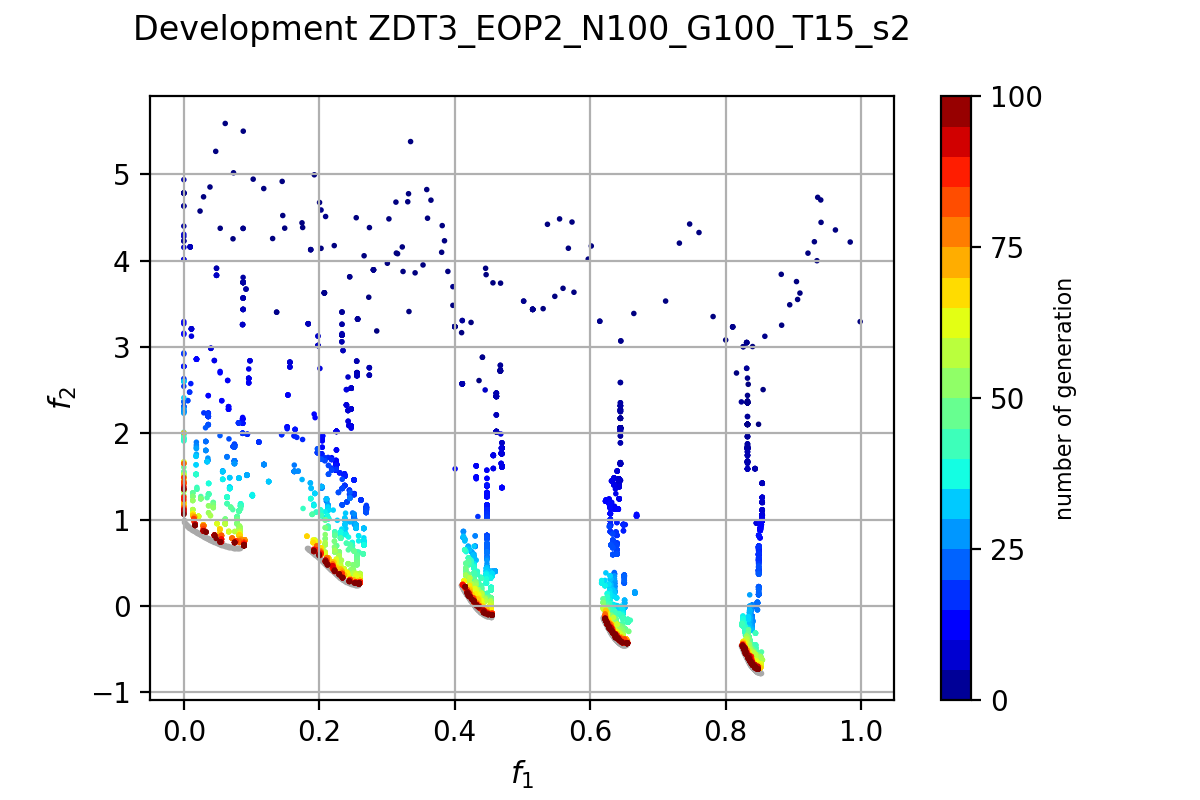
\includegraphics[scale=0.4]{figures/ZDT3_EOP2_N100_G100_T15/s2_dev.png}\\
        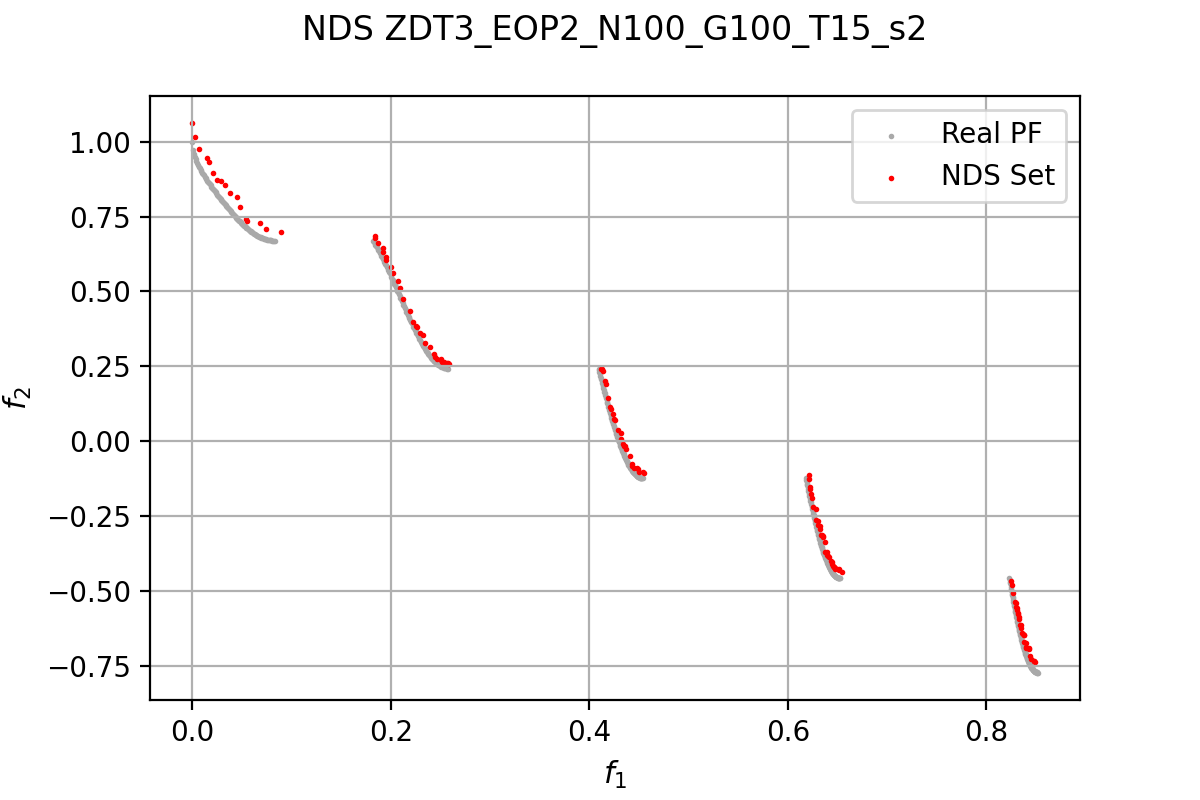
\includegraphics[scale=0.36]{figures/ZDT3_EOP2_N100_G100_T15/s2_nds.png}\\
        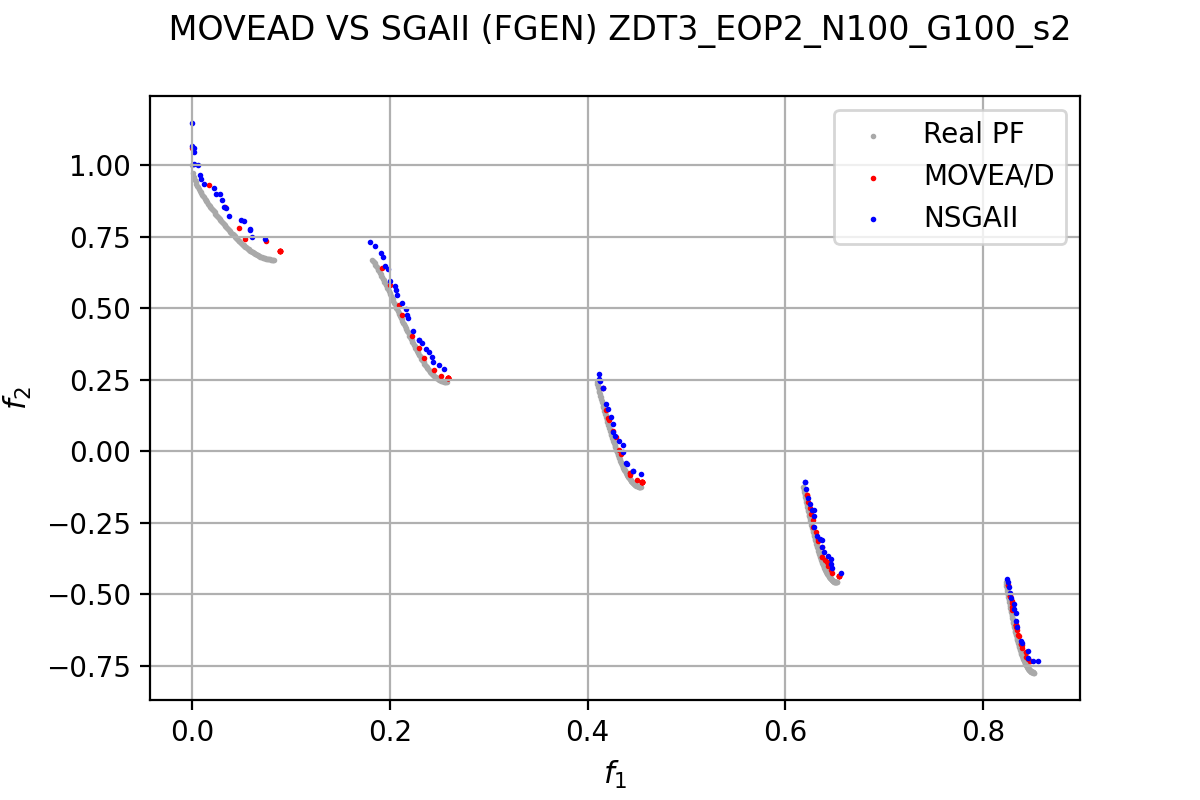
\includegraphics[scale=0.36]{figures/ZDT3_EOP2_N100_G100_T15/s2_comp.png}\\
        \caption{\centering MOEA/D + EOP2 (N100G100)}
        \label{fig:10}
    \end{figure}
\end{minipage} \quad
\begin{minipage}[b]{0.3\linewidth}
\begin{figure}[H]
        \centering
        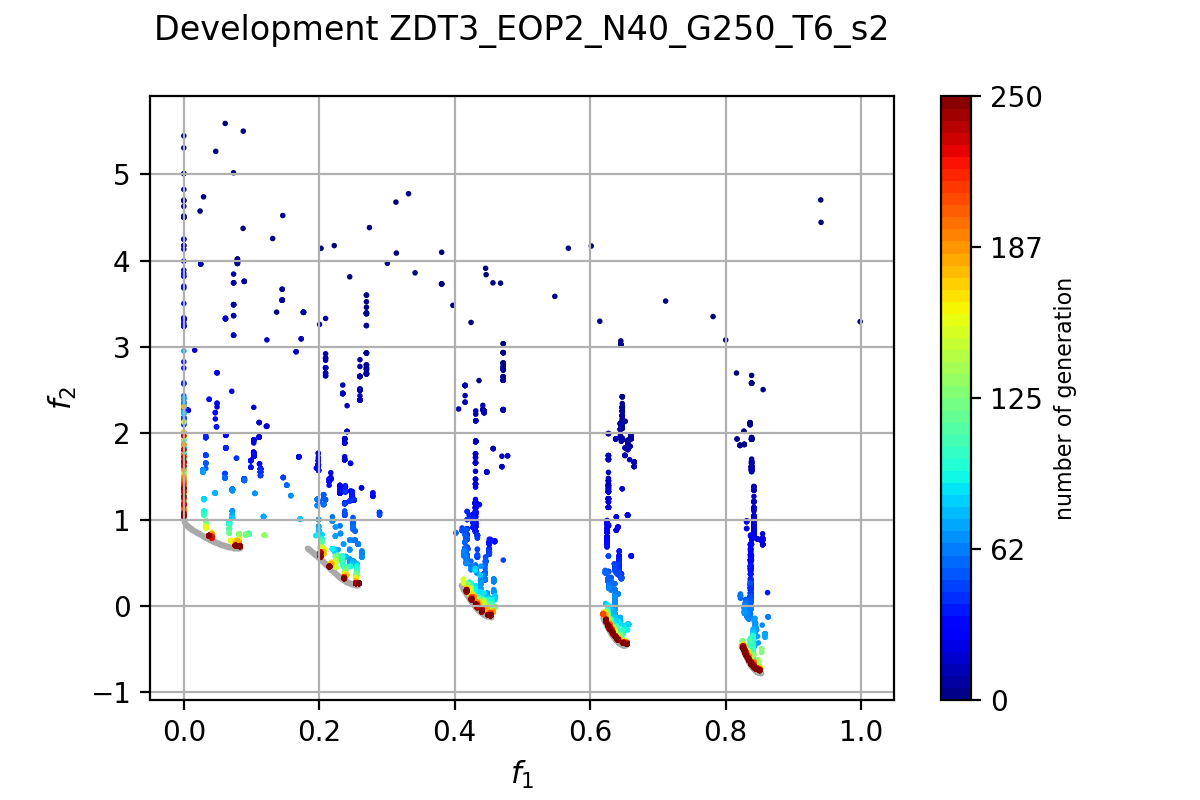
\includegraphics[scale=0.4]{figures/ZDT3_EOP2_N40_G250_T6/s2_dev.png}\\
        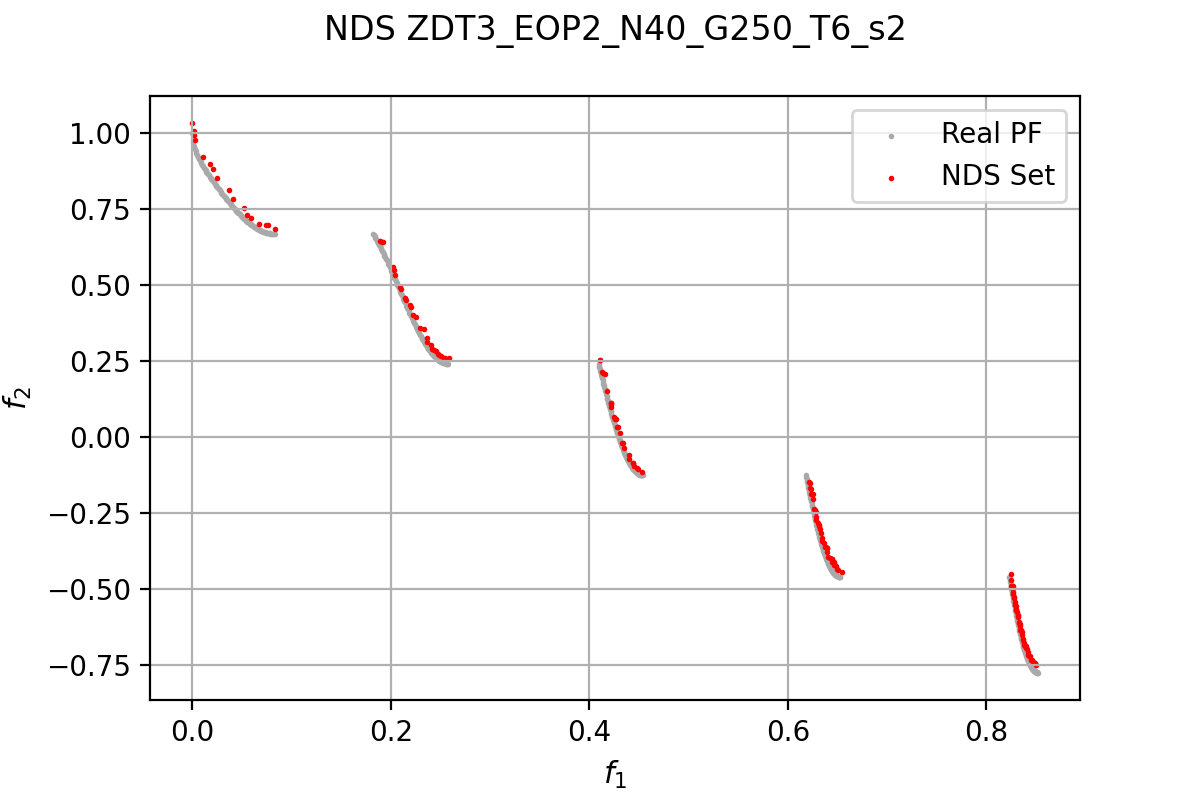
\includegraphics[scale=0.36]{figures/ZDT3_EOP2_N40_G250_T6/s2_nds.png}\\
        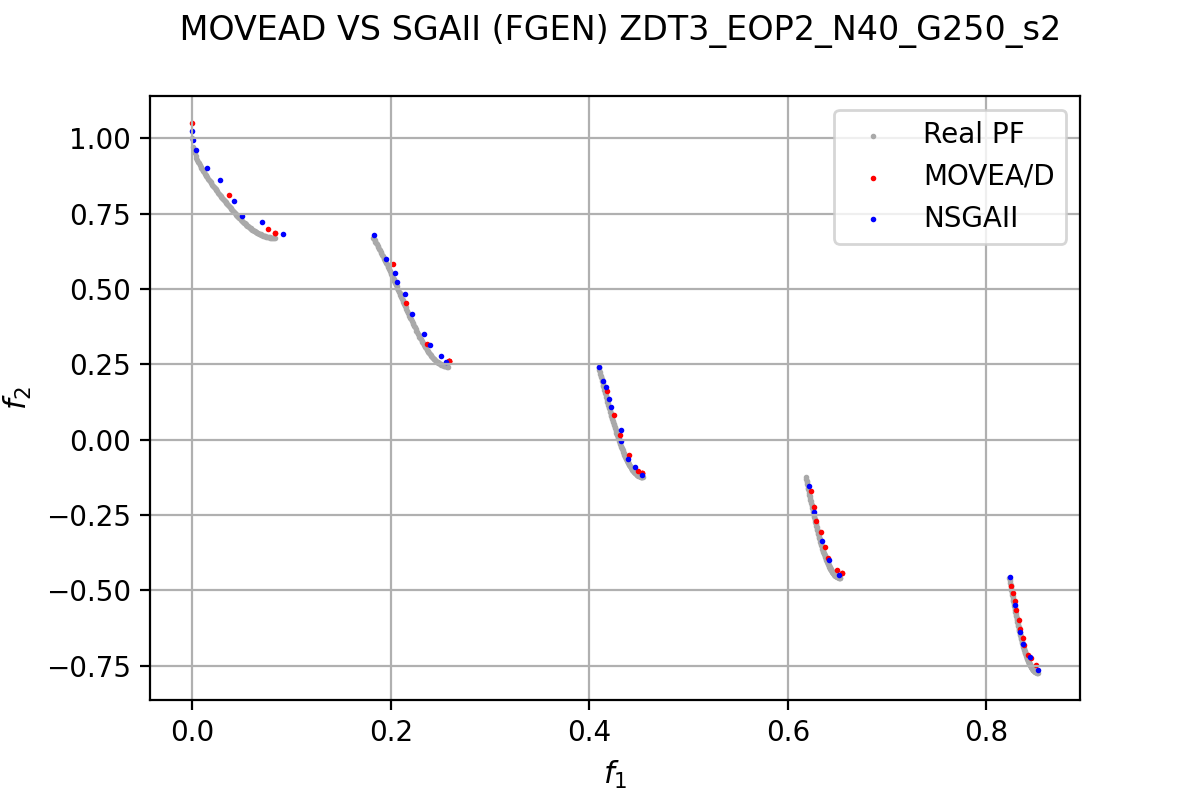
\includegraphics[scale=0.36]{figures/ZDT3_EOP2_N40_G250_T6/s2_comp.png}\\
        \caption{\centering MOEA/D + EOP2 (N40G250)}
        \label{fig:11}
    \end{figure}
\end{minipage} \quad
\begin{minipage}[b]{0.3\linewidth}
    \begin{figure}[H]
        \centering
        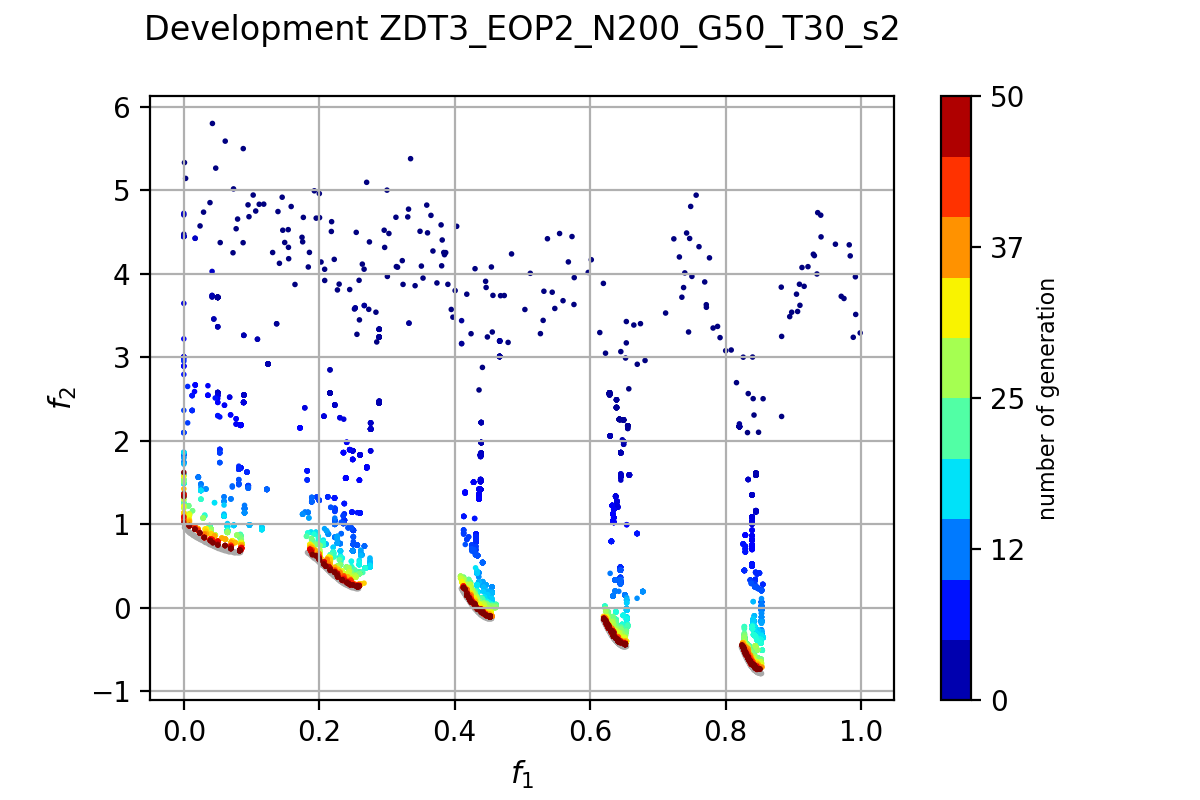
\includegraphics[scale=0.4]{figures/ZDT3_EOP2_N200_G50_T30/s2_dev.png}\\
        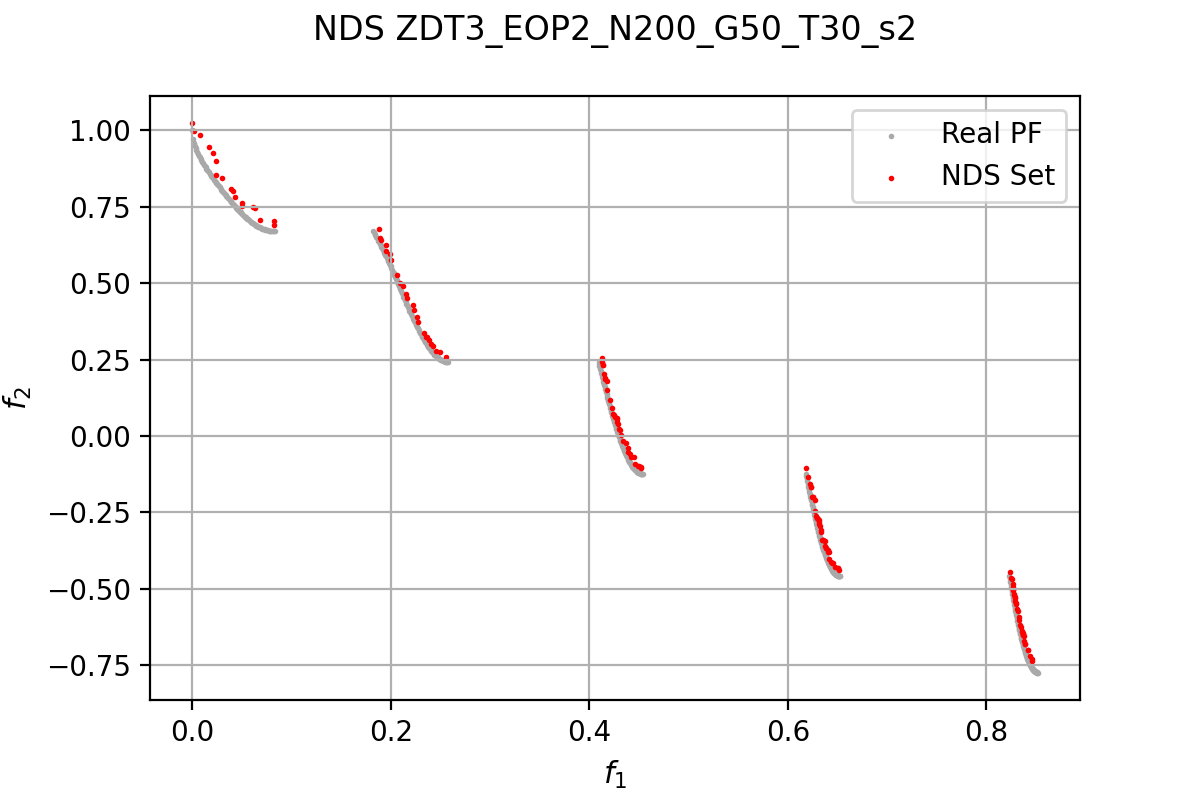
\includegraphics[scale=0.36]{figures/ZDT3_EOP2_N200_G50_T30/s2_nds.png}\\
        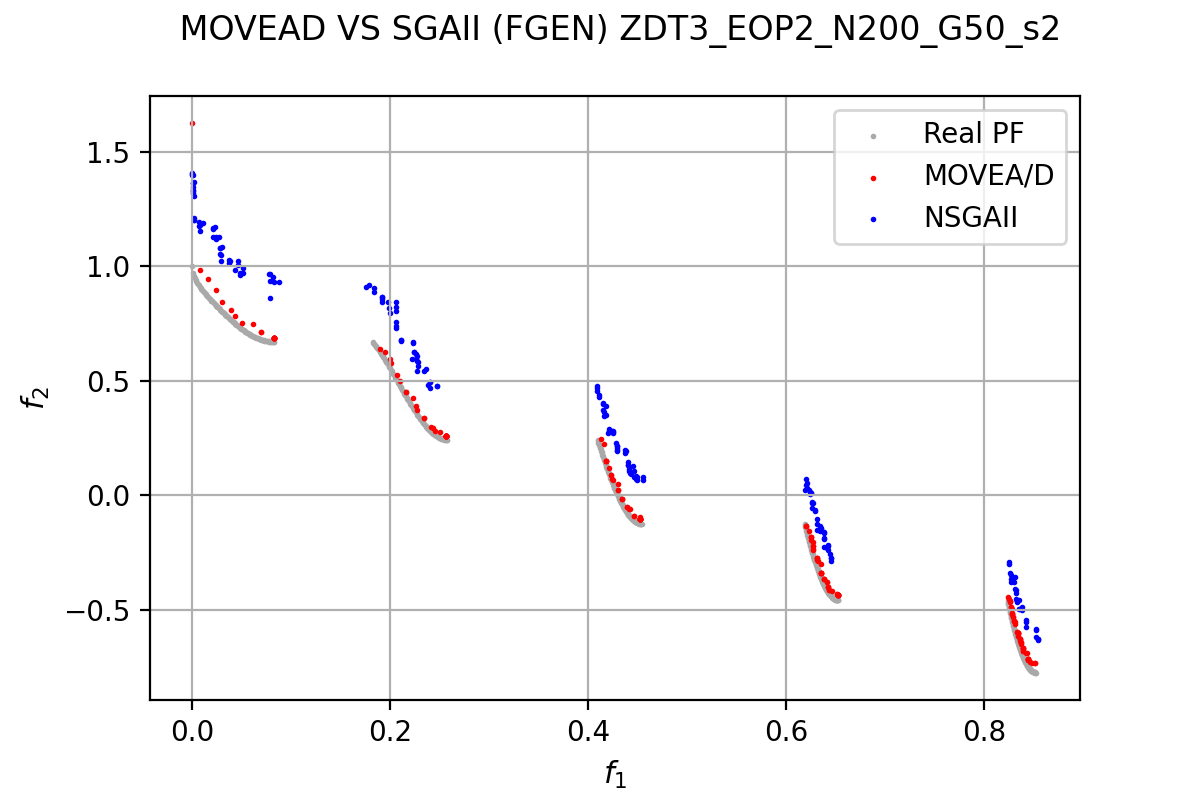
\includegraphics[scale=0.36]{figures/ZDT3_EOP2_N200_G50_T30/s2_comp.png}\\
        \caption{\centering MOEA/D + EOP2 (N200G50)}
        \label{fig:12}
    \end{figure}
    \end{minipage}\\
\end{minipage}\\



Veámos ahora unas gráficas análogas a las presentadas pero para el caso $(G=250, N=40)$ en la \hyperref[fig:11]{\textit{figura 11}} podemos notar que el comportamiento es similar al caso anterior, esto es, como se espera a través de las generaciones las soluciones van aproximándose la convergencia al igual que en el caso anterior sigue siendo es buena, sin embargo se nota que la reducción en el número de subproblemas afecta de manera notable a la dispersión, sobre todo en las últimas generaciones. Sin embargo, si miramos el frente de soluciones no dominadas, vemos que tanto en convergencia (a priori, sin otro algoritmo de referencia) que tanto el grado de convergencia de las soluciones como el grado de dispersión hacen que se aproximen en buena medida al frente real de Pareto, por lo que nos incita a pensar que la pérdida de diversidad debe darse relativamente al final porque existen soluciones buenas a lo largo prácticamente de todo el frente. Si comparamos ahora la última generación con la del algoritmo \textit{NSGA-II} (ejecutado en las mismas condiciones) podemos ver que ahora la superioridad no es tan patente como en el casi anterior y ambos algoritmos alcanzan un grado análogo de convergencia y dispersión (en este último aspecto quizá \textit{NSGA-II} parezca un poco mejor).\\


Y en último lugar comprobemos cuál es el resultado de elevar el número de subproblemas frente al número de generaciones. Dado que según hemos visto hasta ahora lo convergencia suele ser rápida, y que el número de subproblemas favorecerá la diversidad, a priori el comportamiento debería ser satisfactorio. Veámos qué ocurre para el caso $(G=250, N=40)$ en las gráficas presentadas en la \hyperref[fig:12]{\textit{figura 12}}. Podemos notar que la convergencia es bastante buena y la diversidad también permite que en las últimas generaciones se cubran los tramos del frente de manera más o menos uniforme. De hecho, si observamos el diagrama de las soluciones no dominadas podemos notar que, primero el ajuste es ligeramente peor que en los otros casos (normal dado que tiene menos generaciones para tratar de ajustarse) y la cobertura es buena y se reparte de forma más o menos uniforme. Si comparamos con la ejecución del \textit{NSGA-II} en este caso nuestro algoritmo es claramente mejor en convergencia y posiblemente en cobertura. \\

Finalmente vamos a realizar una comparativa entre los tres casos tanto para los frentes de la última generación como para los frentes \textit{NSD}. En la \hyperref[fig:13]{\textit{figura 13}} se muestran las dos gráficas de comparativa de los frente anteriormente indicados. En cuanto a las soluciones de la generación final todas se encuentran bastante superpuestas, quizá la la verde con una menor dispersión pareciendo que un número de subproblemas más elevado proporciona una mejor solución, aunque los resultados no son concluyentes y trataremos de realizar un estudio más profundo con el uso de las métricas. En cuanto al NSD,los resultados no son nada concluyentes, así que intentaremos clarificarlos con el uso de métricas y el correspondiente estudio estadístico de las mismas.\\ 

\begin{center}
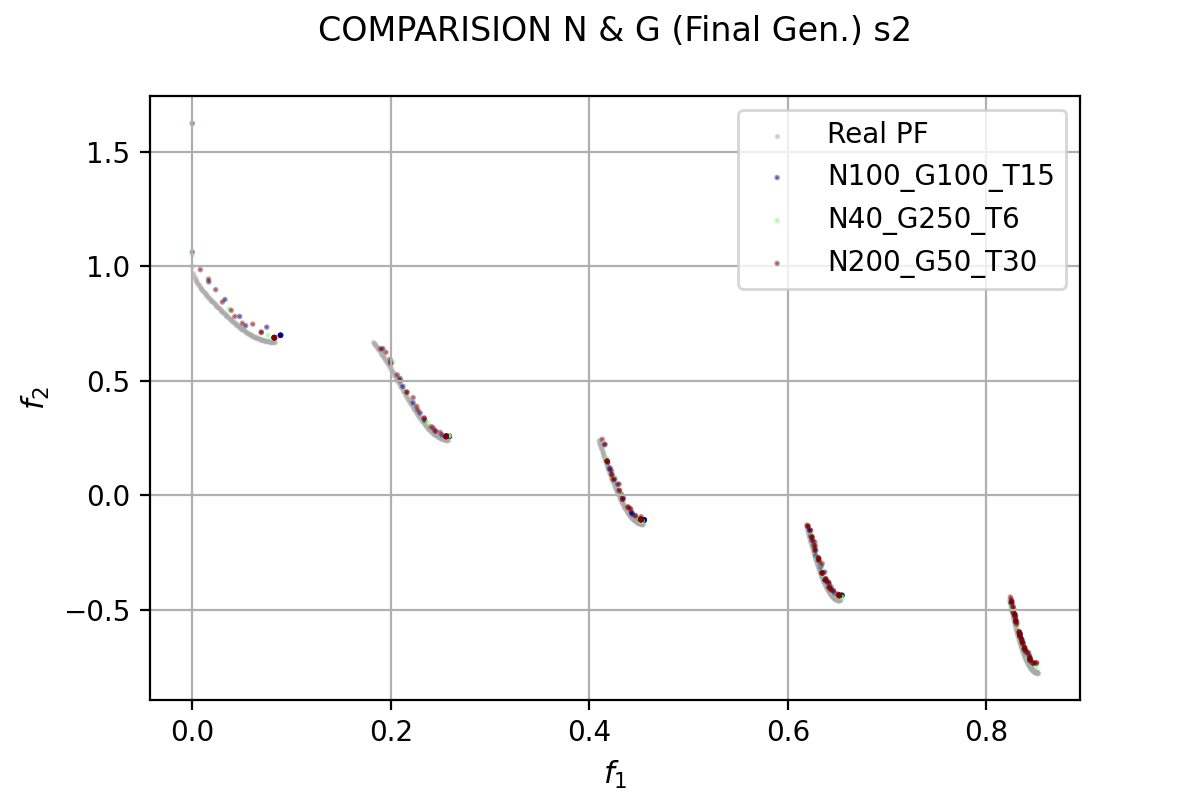
\includegraphics[scale=0.8]{figures/COMPARISIONS_EOP2/GCOMP_FGEN_s2.png}\\
\end{center}
\begin{figure}[H]
\centering
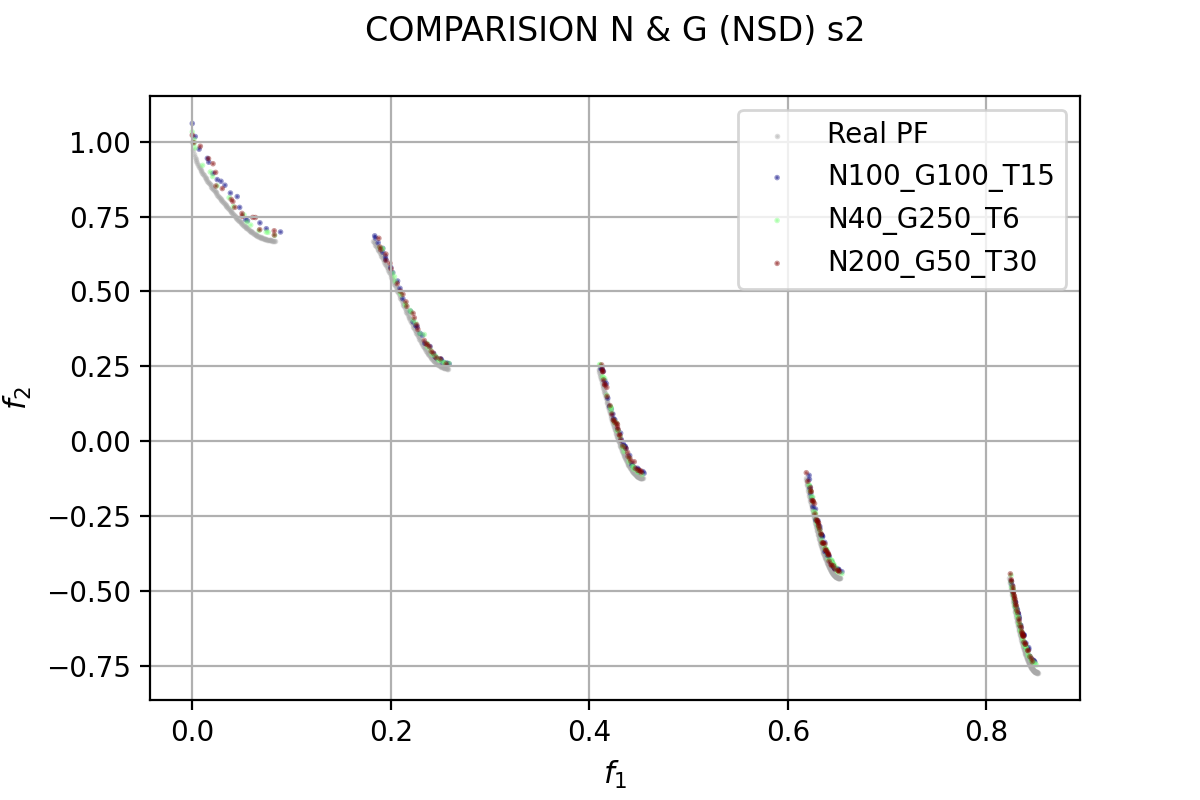
\includegraphics[scale=0.8]{figures/COMPARISIONS_EOP2/GCOMP_NDS_s2.png}\\
\caption{MOEA/D + EOP2. Comparación de casos}
\label{fig:13}
\end{figure}



\subsubsection{Análisis de métricas para 10000 ev.}

Presentado el estudio preliminar anterior vamos a tratar de profundizar para exclarecer y llevar a cabo una discusión más profunda de los casos anteriores. Para ello realizaremos un estudio de algunas métricas para los casos ya presentados. Tales métricas corresponden al hipervolumen, espaciado y cover set.\\

Comencemos viendo algunas gráficas asociadas a las métricas para los casos planteados en el apartado anterior. En la \hyperref[fig:14]{figura 14} se muestra la evolución de hipervolumen y el espaciado en durante las distintas generaciones para 10 ejecuciones del algoritmo. Podemos observar que en todos los casos  el desarrollo del hipervolumen se comporta de manera bastante uniforme para todas las ejecuciones, sin embargo en el primer caso el espaciado sí varía considerablemente desde menos de 0.04 para algunas ejecuciones hasta casi 0.10 en otras.\\

Aunque no es posible hacer un análisis conjunto del hipervolumen (ya que el punto de referencia para su cálculo es distinto en cada caso) sí podemos destacar la rápida convergencia del algoritmo, menos clara que para EOP1 (hecho que destacamos también en el estudio preliminar) y el aparente estancamiento final, por lo que es preferible primar el número de subproblemas frente al número de generaciones (en valores razonables)como sugiere también el comportamiento del espaciado, que para el segundo y el tercer caso se comporta de manera más iniforme, para ambos con valores entre 0.01 y 0.03\\


\begin{figure}[H]
\centering
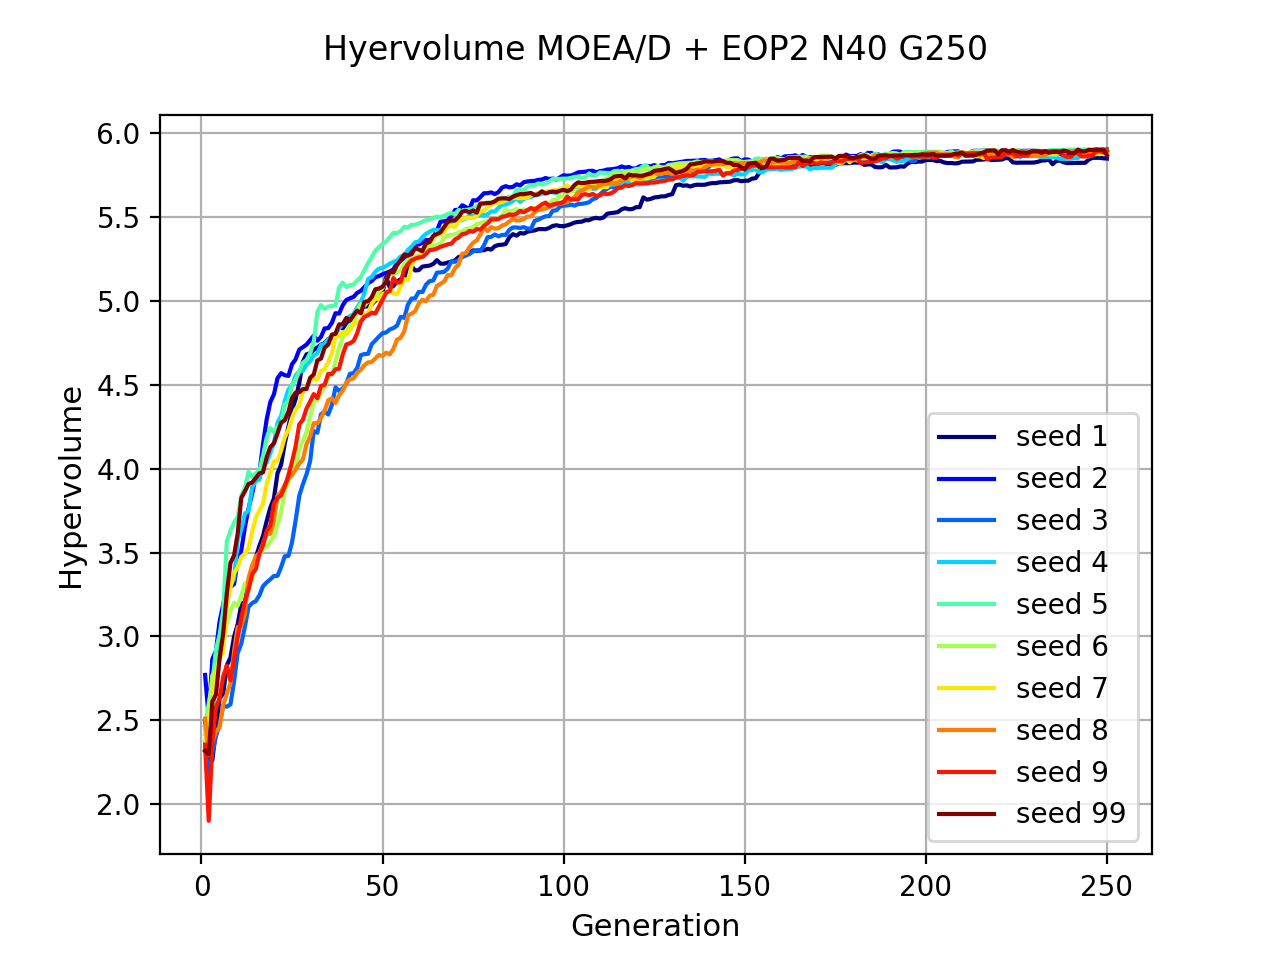
\includegraphics[scale=0.5]{figures/METRICS_EOP2/Hypervol_N40_G250.png}\quad 
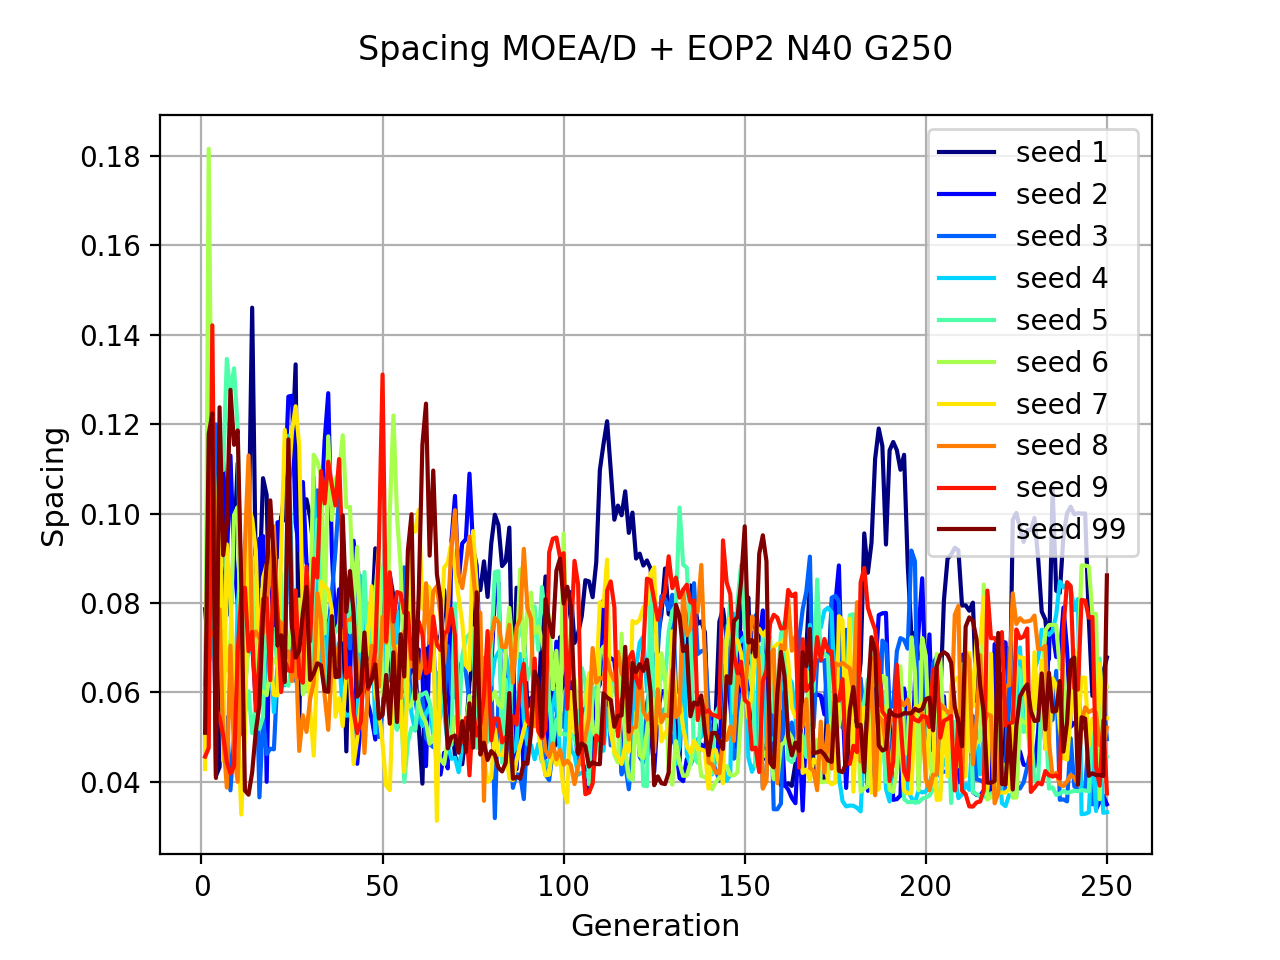
\includegraphics[scale=0.5]{figures/METRICS_EOP2/Spacing_N40_G250.png}\\
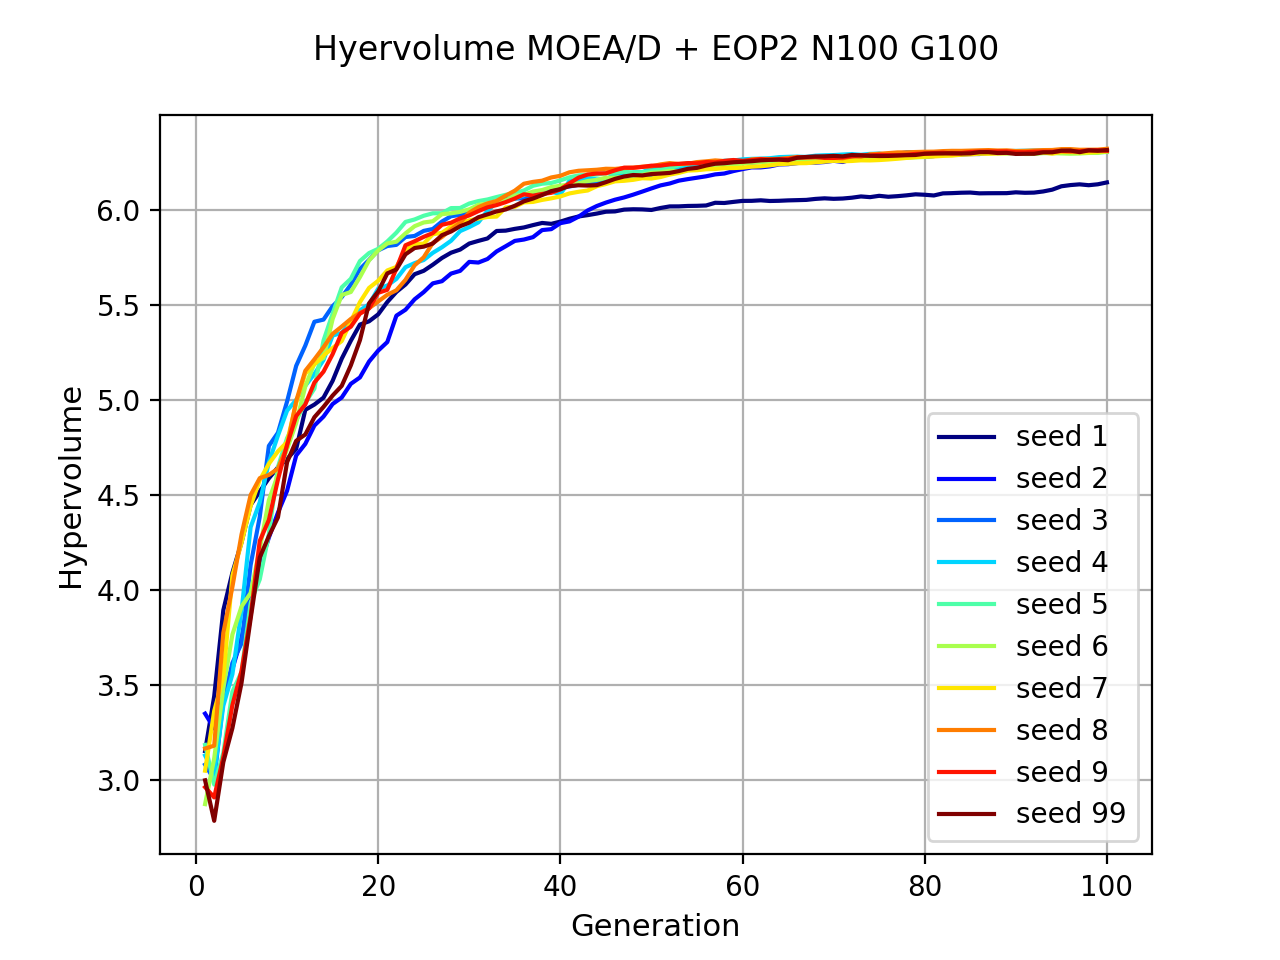
\includegraphics[scale=0.5]{figures/METRICS_EOP2/Hypervol_N100_G100.png} \quad 
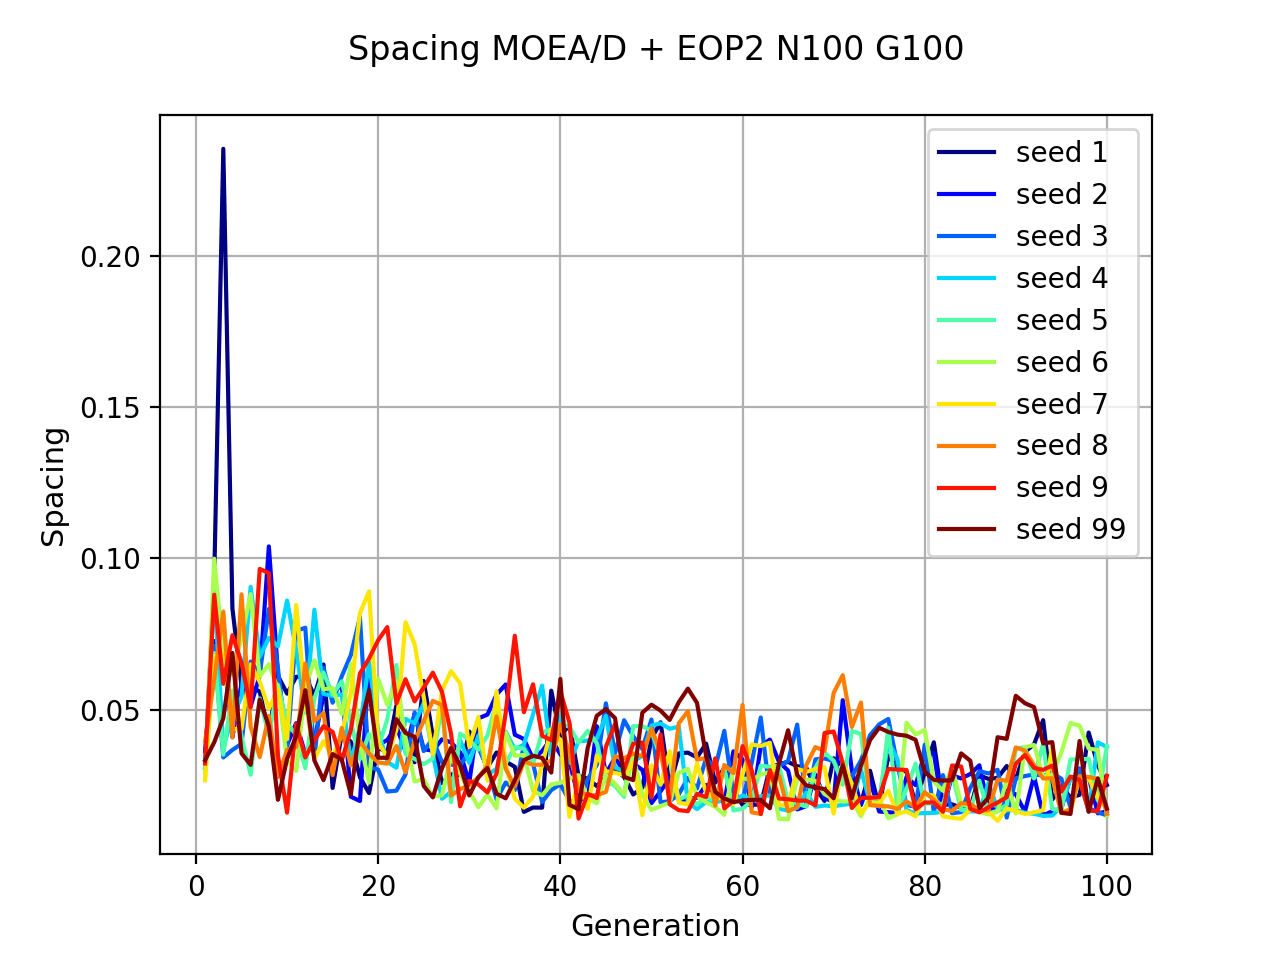
\includegraphics[scale=0.5]{figures/METRICS_EOP2/Spacing_N100_G100.png}\\
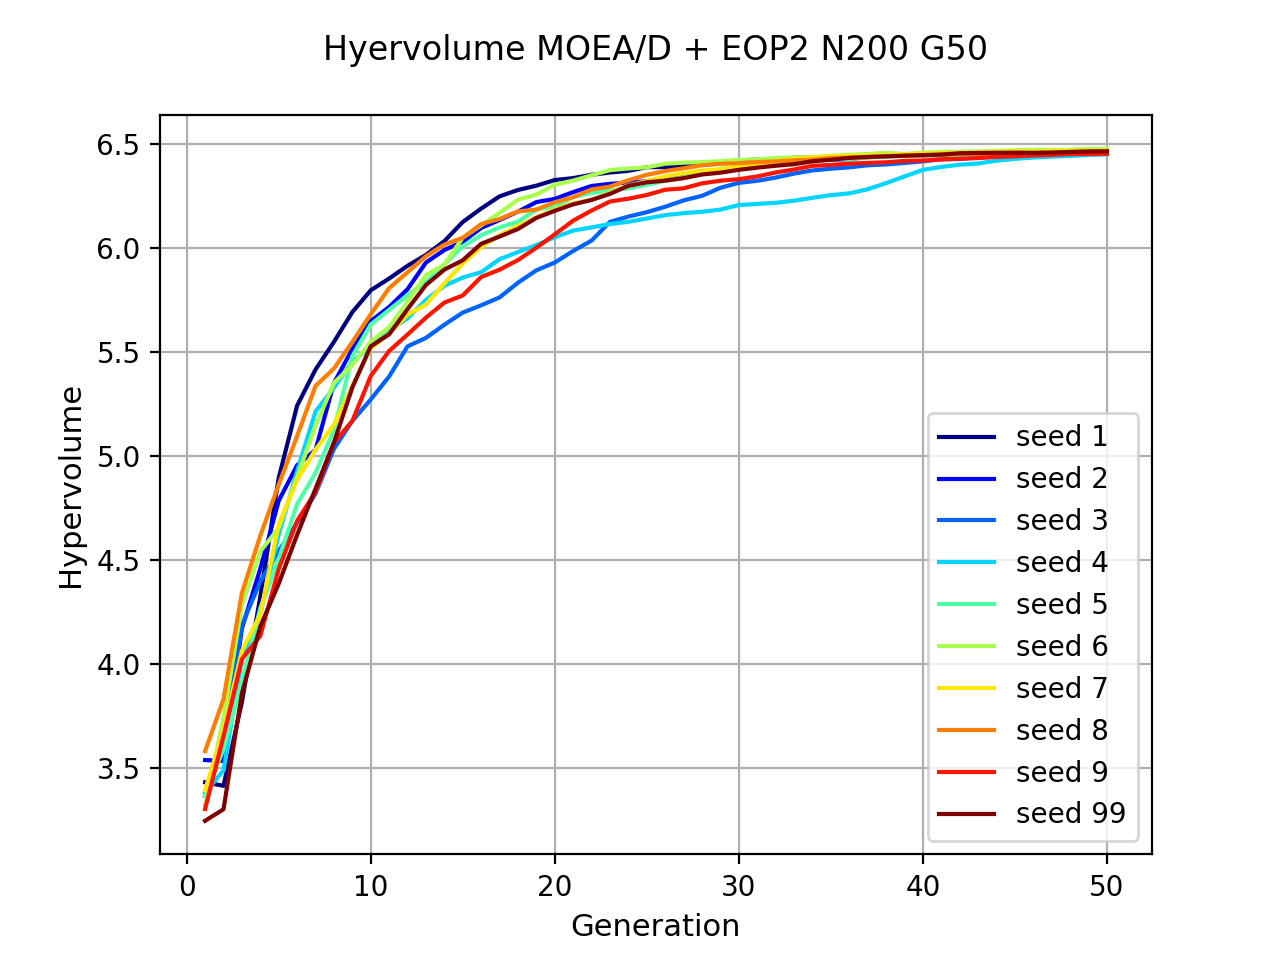
\includegraphics[scale=0.5]{figures/METRICS_EOP2/Hypervol_N200_G50.png}\quad 
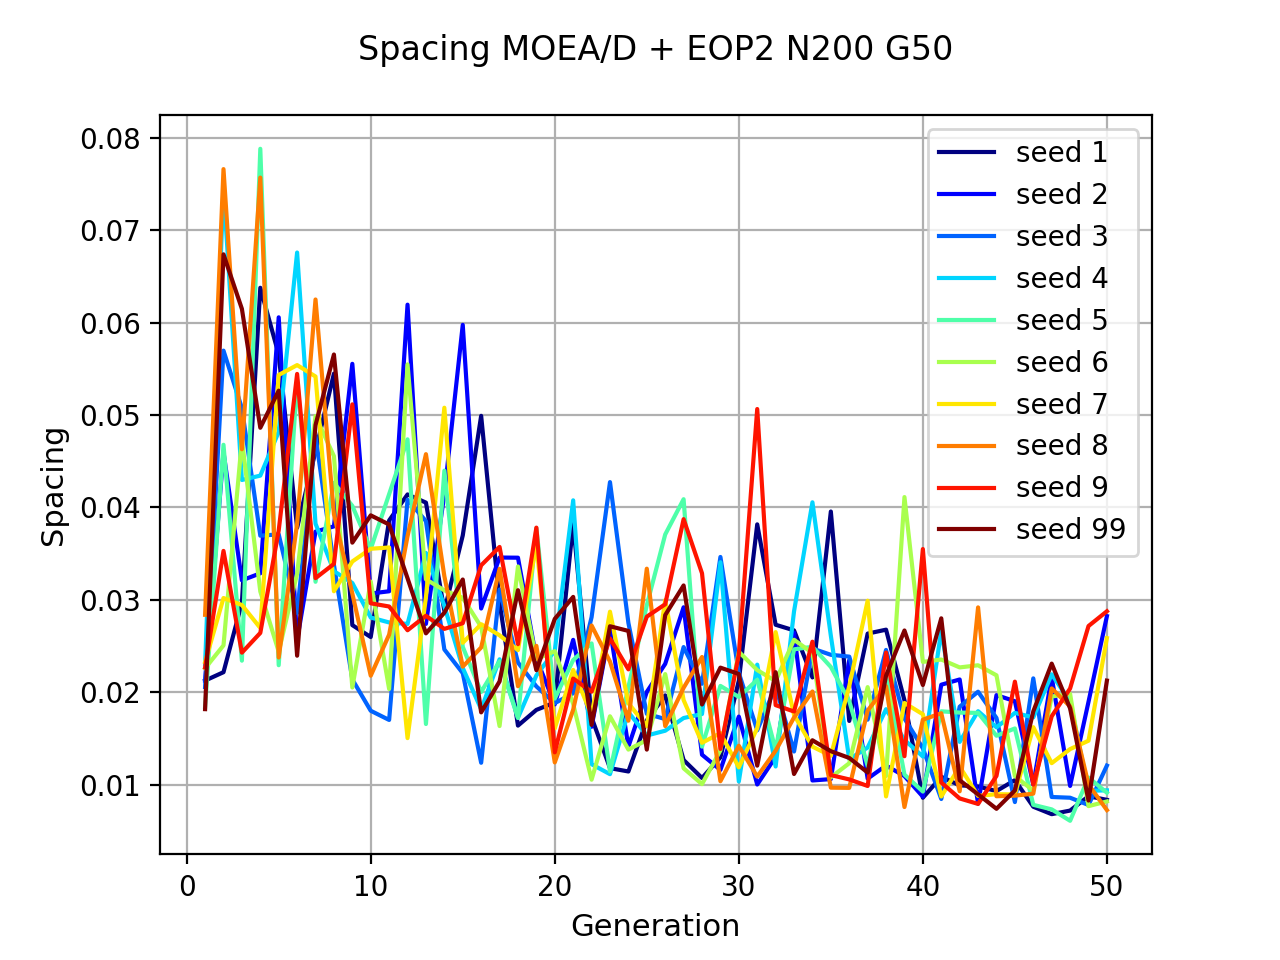
\includegraphics[scale=0.5]{figures/METRICS_EOP2/Spacing_N200_G50.png}\\
\caption{MOEA/D + EOP2. Méticas para 10000 EV}
\label{fig:14}
\end{figure}


\begin{figure}[H]
\centering
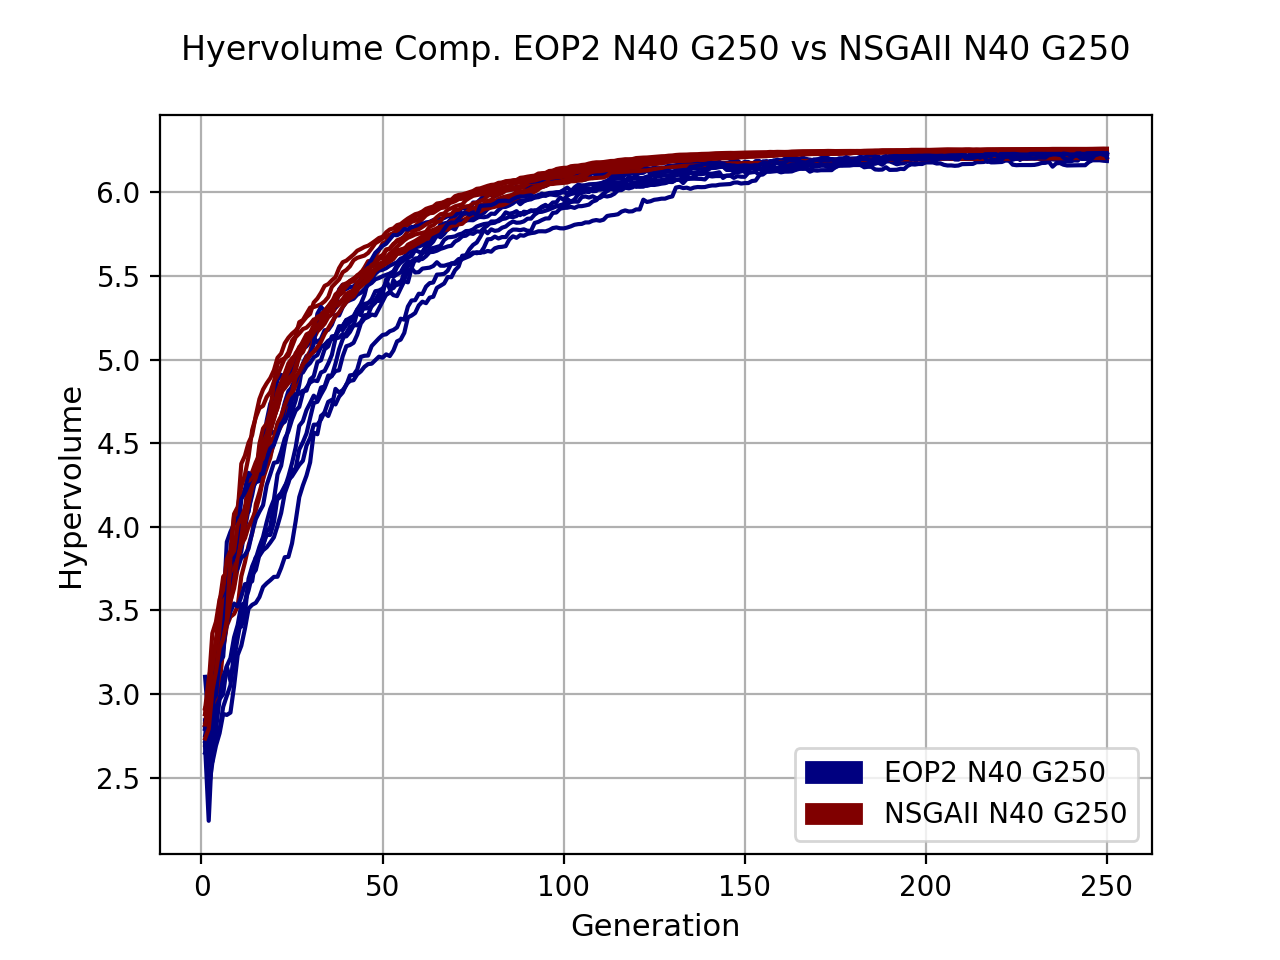
\includegraphics[scale=0.35]{../METRICS_PLOTS/Hypervol_COMP_EOP2N40G250_NSGAIIN40G250.png}
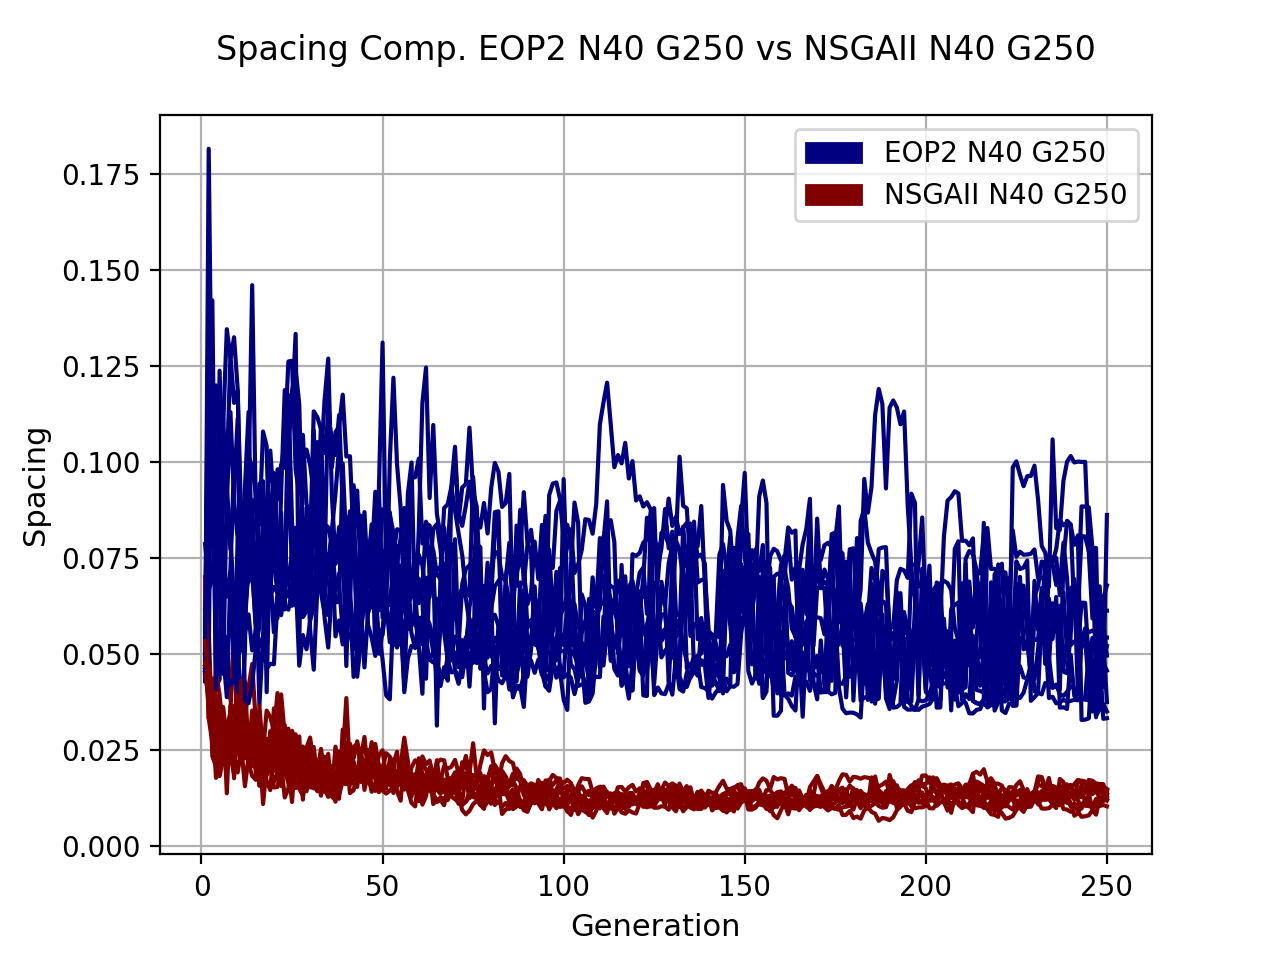
\includegraphics[scale=0.35]{../METRICS_PLOTS/Spacing_COMP_EOP2N40G250_NSGAIIN40G250.png}
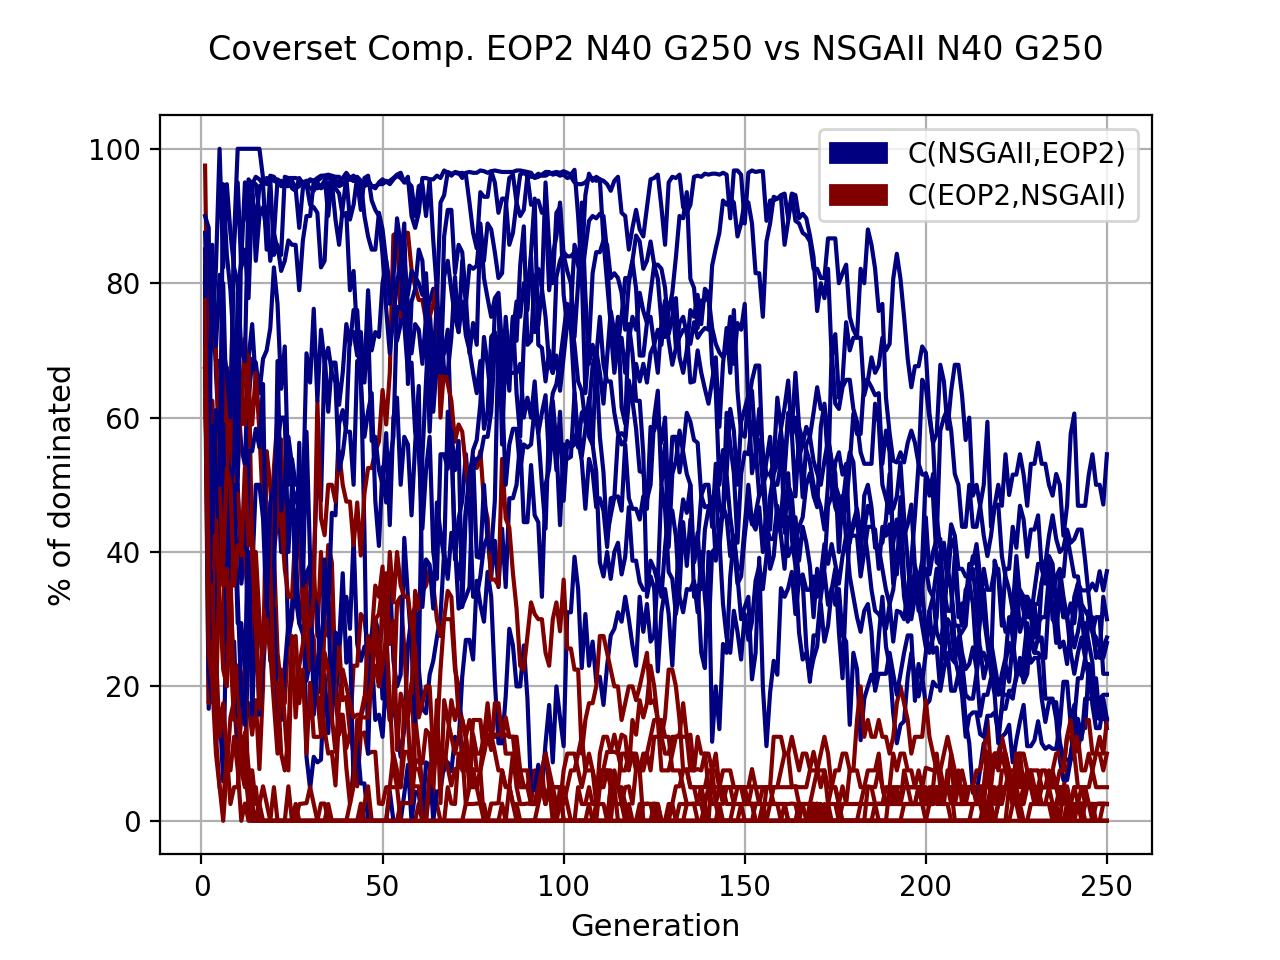
\includegraphics[scale=0.35]{../METRICS_PLOTS/CoverSet_COMP_EOP2N40G250_NSGAIIN40G250.png}\\
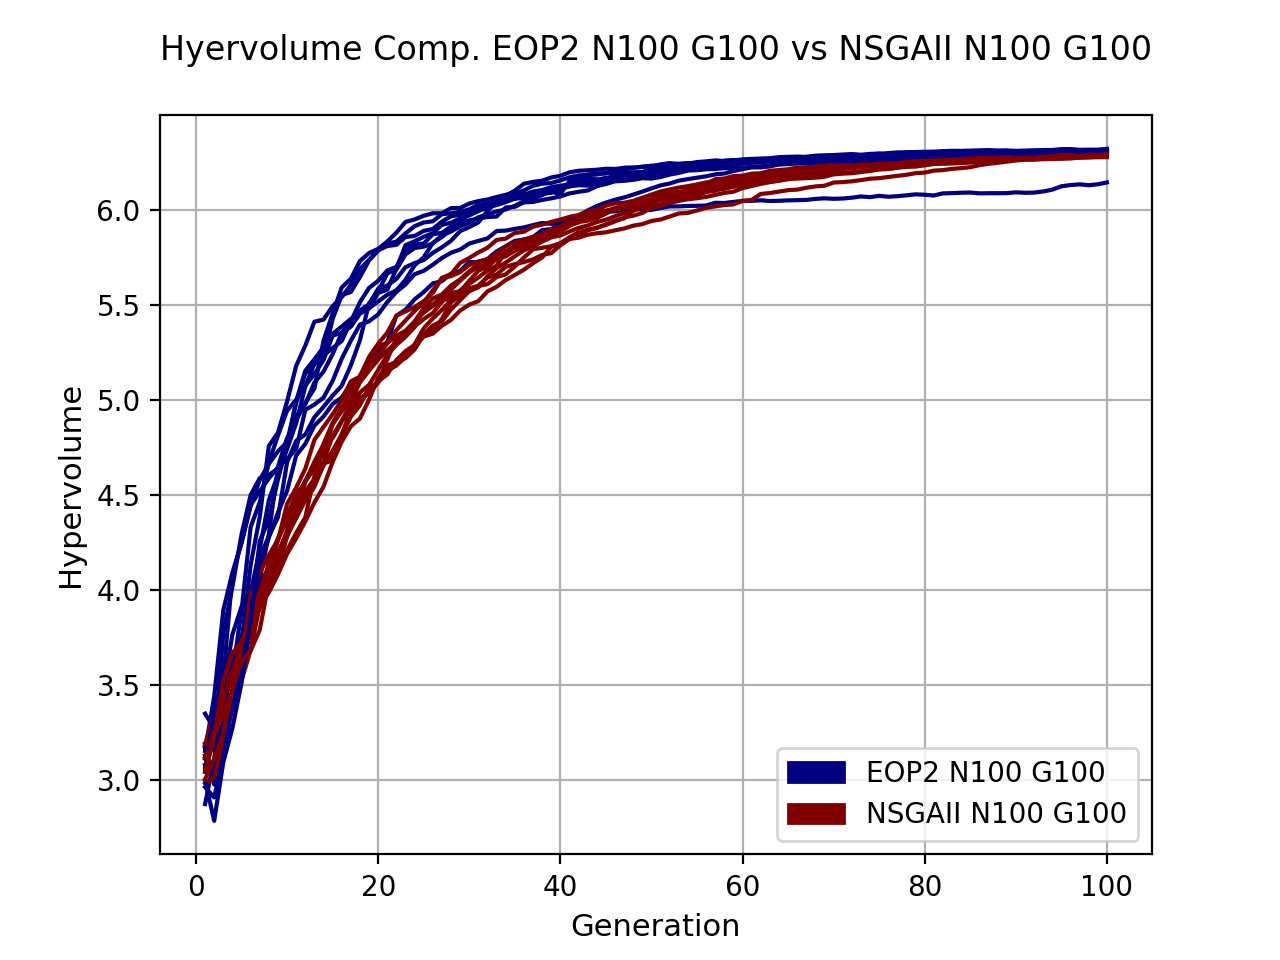
\includegraphics[scale=0.35]{../METRICS_PLOTS/Hypervol_COMP_EOP2N100G100_NSGAIIN100G100.png}
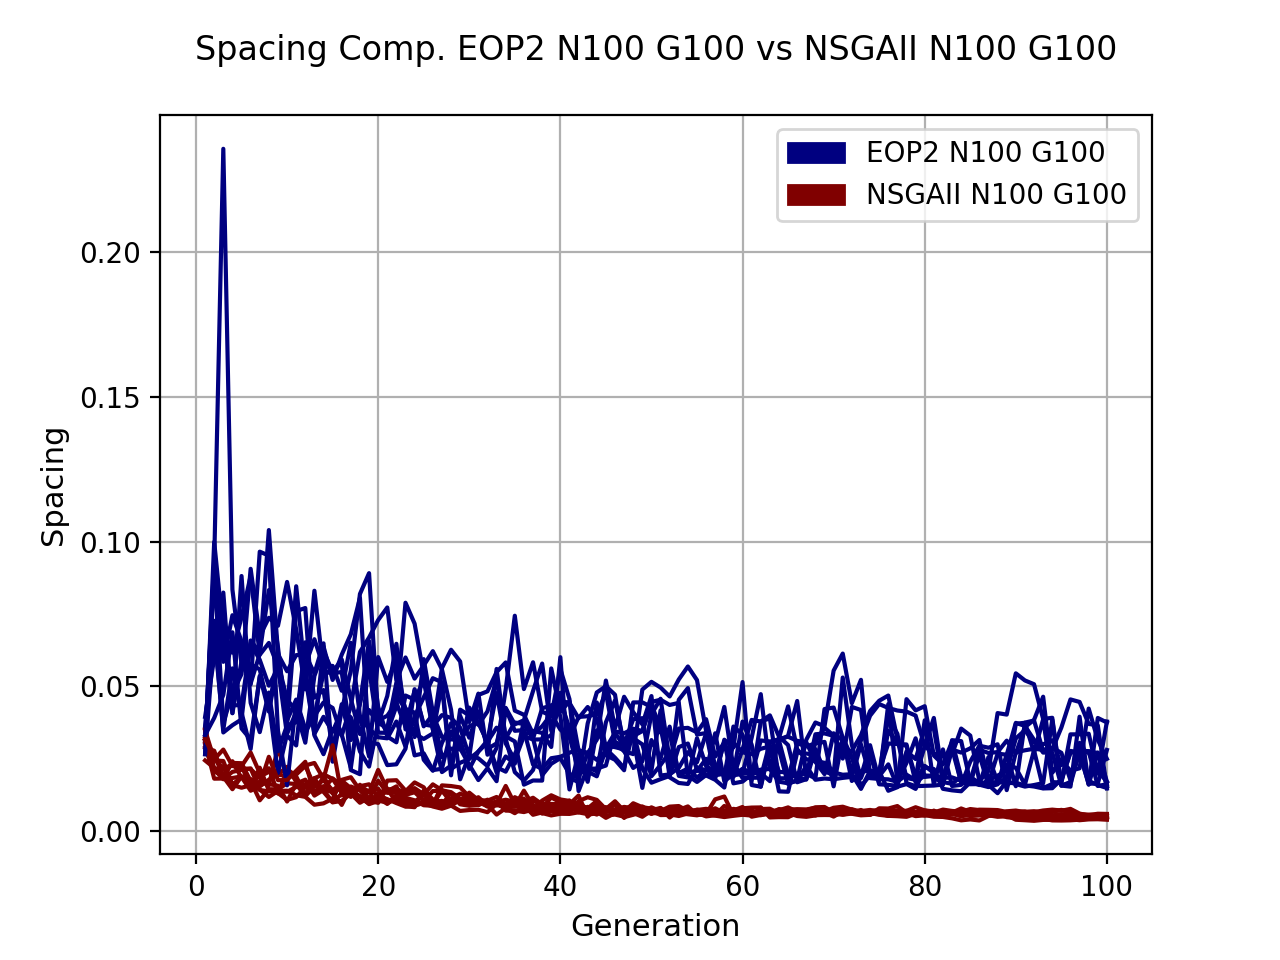
\includegraphics[scale=0.35]{../METRICS_PLOTS/Spacing_COMP_EOP2N100G100_NSGAIIN100G100.png}
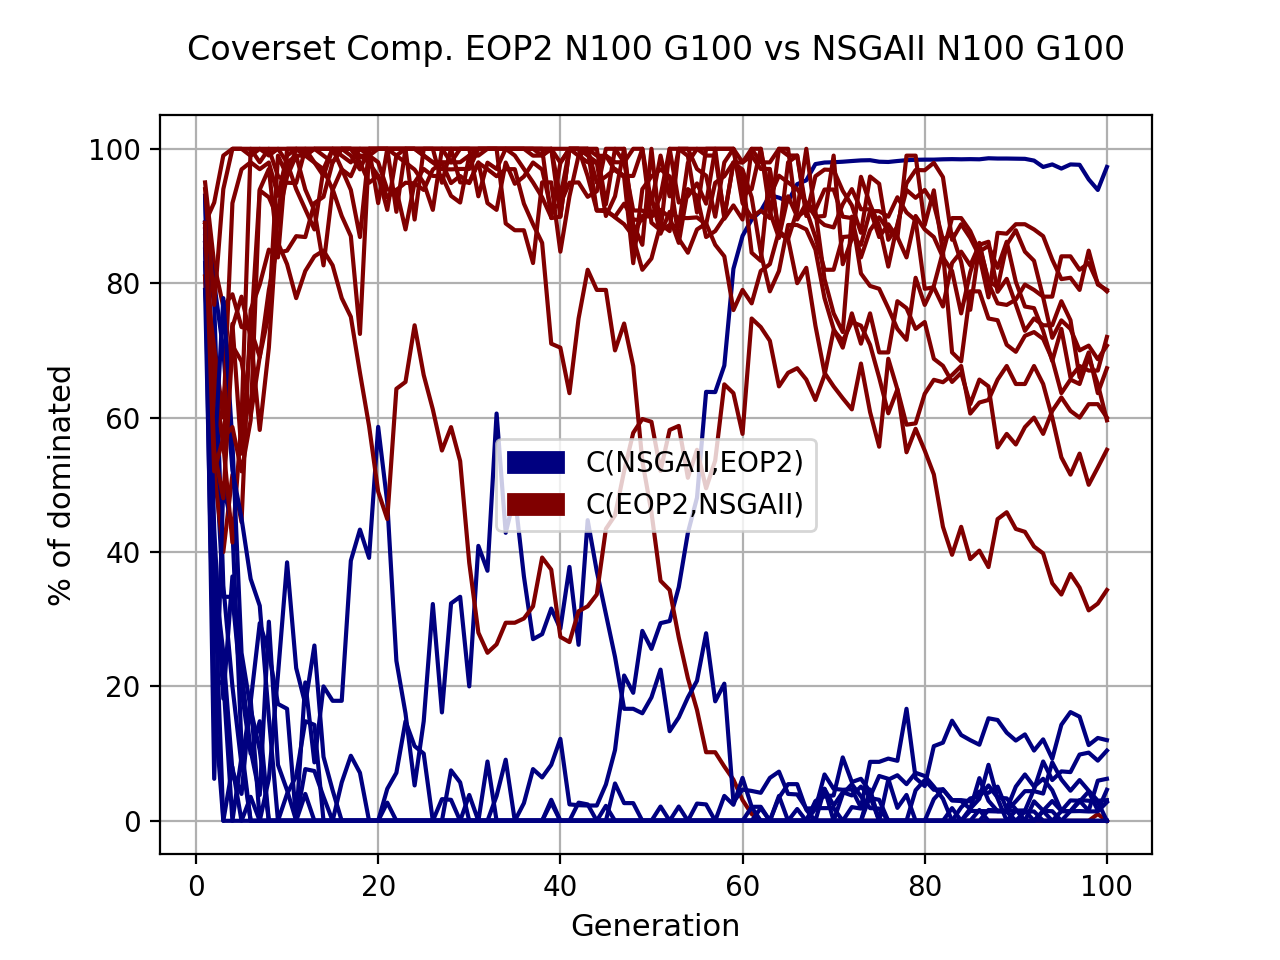
\includegraphics[scale=0.35]{../METRICS_PLOTS/CoverSet_COMP_EOP2N100G100_NSGAIIN100G100.png}\\
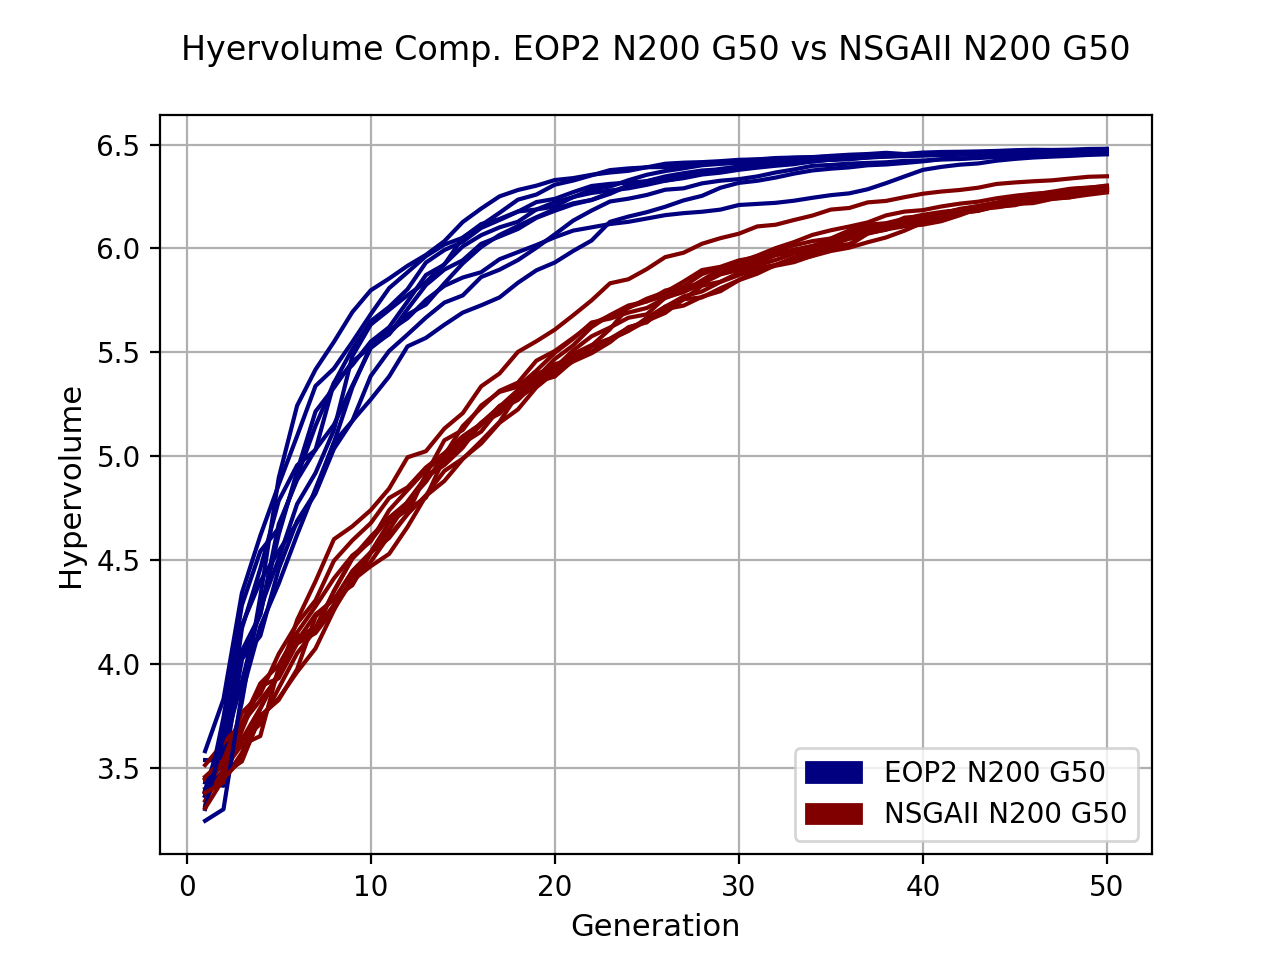
\includegraphics[scale=0.35]{../METRICS_PLOTS/Hypervol_COMP_EOP2N200G50_NSGAIIN200G50.png}
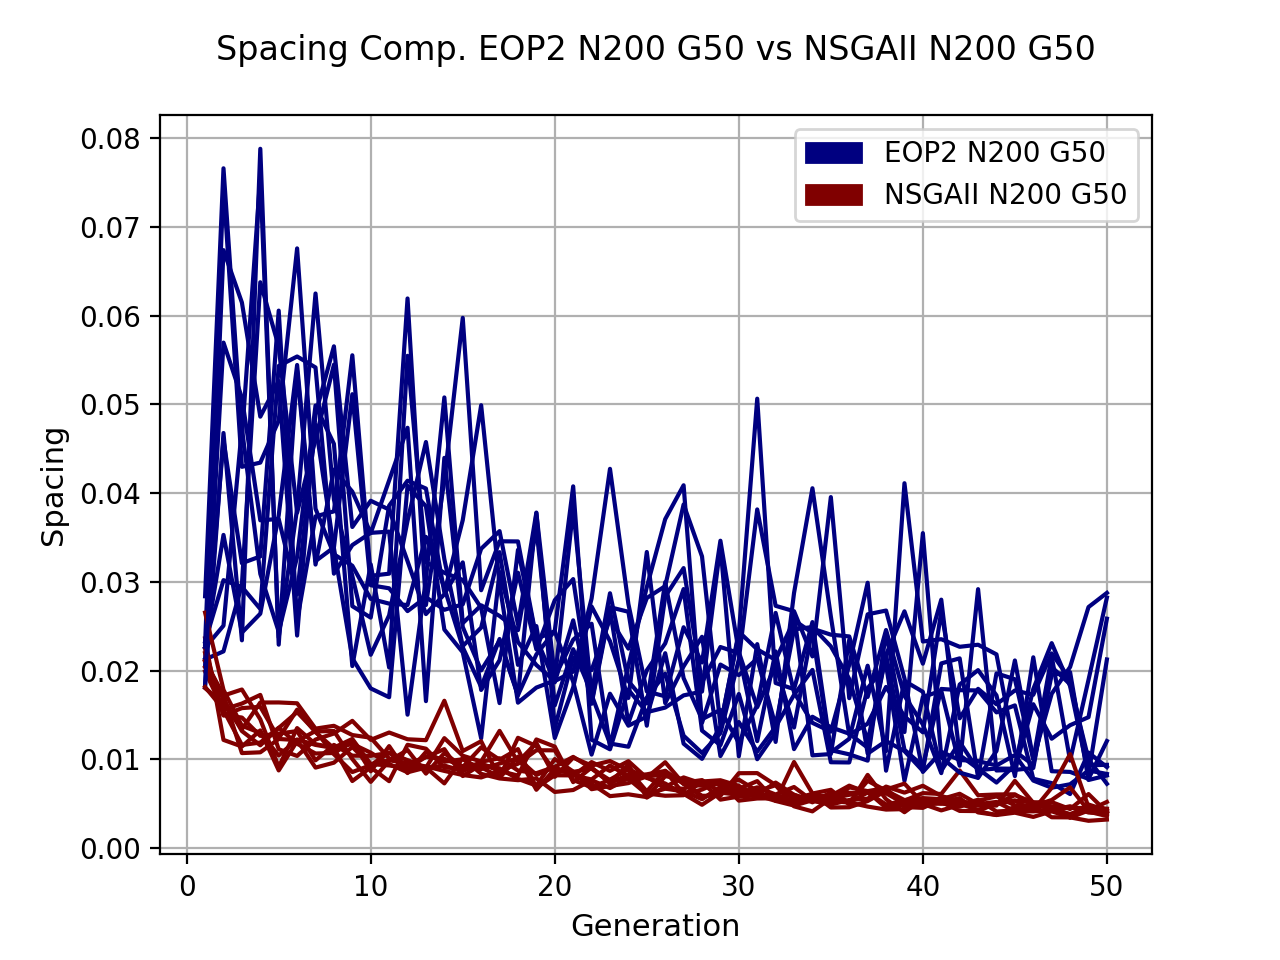
\includegraphics[scale=0.35]{../METRICS_PLOTS/Spacing_COMP_EOP2N200G50_NSGAIIN200G50.png}
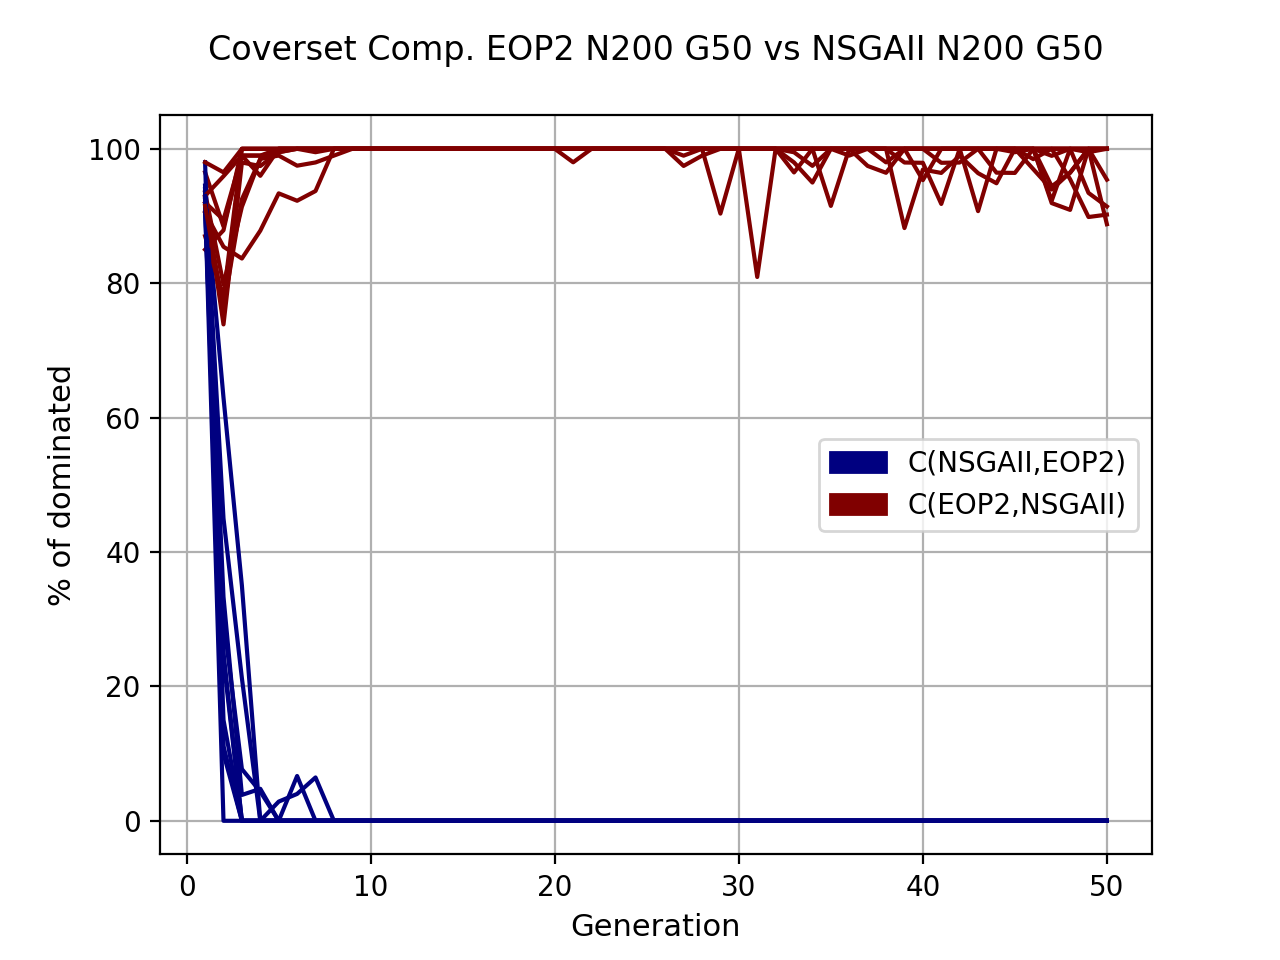
\includegraphics[scale=0.35]{../METRICS_PLOTS/CoverSet_COMP_EOP2N200G50_NSGAIIN200G50.png}\\
\caption{MOEA/D + EOP2. Comparación de métricas con NSGAII para 10000 EV.}
\label{fig:15}
\end{figure}

A continuación presentaremos algunas gráficas comparativas del comportamiento del algoritmo frente a \textit{NSGAII}. En la \hyperref[fig:15]{figura 15} se muestran las graficas con dichas comparativas en las que podemos notar que en todos los casos el espaciado en el algoritmo \textit{NSGAII} se comporta mejor que en algoritmo propuesto mientras que el hipervolumen para el caso ($N=40$, $G=250$) es favorable al algoritmo \textit{NSGAII} y favorable a nuestro algoritmo para el resto de los casos. Como vimos en el estudio preliminar el algoritmo, con los suficientes subproblemas, sí suele converger a soluciones mejores que el algoritmo \textit{NSGAII} pero también suele tender a concentrar más las soluciones.\\

Sin embargo si comprobamos la métrica cover set, sí podemos ver que en el primer caso ninguno de los frentes es dominado más de un 50\% por el otro en la mayoría de las ejecuciones, pero aún así \textit{NSGAII} tiende a quedar por debajo. Para el segundo y el tercer caso ($N100$ y $N200$) el algoritmo propuesto tiende a dominar al \textit{NSGAII}. Más concretamente para el segundo caso en casi todas las ejecuciones el frente del algoritmo \textit{NSGAII} quedó dominado por el de \textit{MOEA/D + EOP2} entre el 50\% y el 80\% de sus puntos, mientras que el frente de  \textit{NSGAII} domina al \textit{MOEA/D + EOP2} en menos de un 20\% en prácticamente todas de las ejecuciones. En el último caso, los resultados sí son claros, el frente de \textit{NSGAII} queda dominado por el de nuestro algoritmo en más de un 90\% en todas las ejecuciones mientras que el caso contrario no es apreciable para ningún punto de ninguna de las ejecuciones (en más de 1\% o 2\%). De forma que queda patente los resultados que ya comentamos para el operador EOP1 pero que en este caso se manifiestan con mayor relevancia, la cantidad de subproblemas es mucho más beneficiosa que la cantidad de generaciones.\\

Aunque en este apartado no hemos realizado (explícitamente) un análisis de las soluciones (población final y NSD) en el último apartado de esta sección presentaremos una comparativa conjunta de las últimas generaciones y de los conjuntos no dominados (NSD) para todos los casos y todos los algoritmos.	\\

\noindent\textbf{EXPERIMENTACIÓN PARA 4000 EVALUACIONES}\\

Ya presentamos para 10000 evaluaciones el comportamiento del algoritmo es adecuado, esto es, a través de las generaciones los individuos se aproximan al frente. No vamos a volver a presentarlo para el caso de 4000 evaluaciones, pues sigue lógicamente el mismo esquema (en los apéndices se presentan las gráficas que atestiguan lo expuesto). Por tanto pasaremos directamente a evaluar las métricas y a razonar directamente sobre los resultados obtenidos en dicho análisis.  \\

En la \hyperref[fig:16]{figura 16} se presentan las gráficas del desarrollo del hypervolumen y el espaciado para cada uno de los casos coniderados en las 4000 evaluaciones en contreto $(N=40, G=100)$, $(N=80, G=50)$, $(N=100, G=40)$. Como podemos apreciar el comportamiento es similar a los presentados para las 10000 evaluaciones, pero sin embargo es notable el espacio de mejora del algoritmo dado el estado de crecimiento de la curva en todos los casos, lo que parece indicar que más iteraciones y más subproblemas sí serían útiles para la mejora del algoritmo, al contrario que en EOP1 no parece haberse alcanzado el estancamiento. También es notable la gran variabilidad del espaciado dada la falta de subproblemas y generaciones, disminuyendo dicha variabilidad sensiblemente con el aumento de los subproblemas, sobre todo en el tercer caso.\\

Si realizamos una comparativa (al igual que en el caso de 10000 ev) con el algoritmo \textit{NSGAII} obtenemos conclusiones sensiblemente distintas a las presentadas para 10000 evaluaciones y para EOP1, no para el espaciado en el que \textit{NSGAII} supera (valor más bajo) a nuestro algoritmo, aunque sí se denota una notable mejora con el aumento de los subproblemas. Pero en el caso del hipervolumen en el primer caso $(N=40, G=100)$ \textit{NSGAII} supera a nuesto algoritmo en prácticamente la totalidad de las ejecuciones, mientras que en el segundo y tercer caso nuestro algoritmo consigue superarlo en este aspecto. En cuanto al cover set, para el caso $N=40$ más del 50\%   del frente (final) de nuestro algoritmo es dominado por el de \textit{NSGAII} en prácticamente todas las ejecuciones, mientras que apenas un 8\% del frente de nuestro algoritmo domina al competidor. En los otros dos casos el cover set es mucho más claro de forma que para ambos casos en buena parte de las ejecuciones más del 75\% del frente es dominado por el frente final de nuestro algoritmo, mientras que para pocas ejecuciones se produce una dominancia de \textit{NSGAII} en más de un 1\% o 2\%.\\

De todo ello destacamos la bondad de nuestro algoritmo en cuanto a la convergencia, no tanto para el espaciado (sobre todo si consideramos la última generación, si consideramos el frente NSD veremos que el espaciado mejora notablemente, presentado en la comparativa final de la \hyperref[table:1]{tabla 1}) y en cuanto al cover set, con el número adecuado de subproblemas (mejor que de generaciones) nuestro algoritmo domina practicamente en su totalidad a \textit{NSGAII}. Sí hemos de destacar que EOP se comportaba mejor ante la falta de generaciones (esto es su convergencia era más rápida). \\

\begin{figure}[H]
\centering
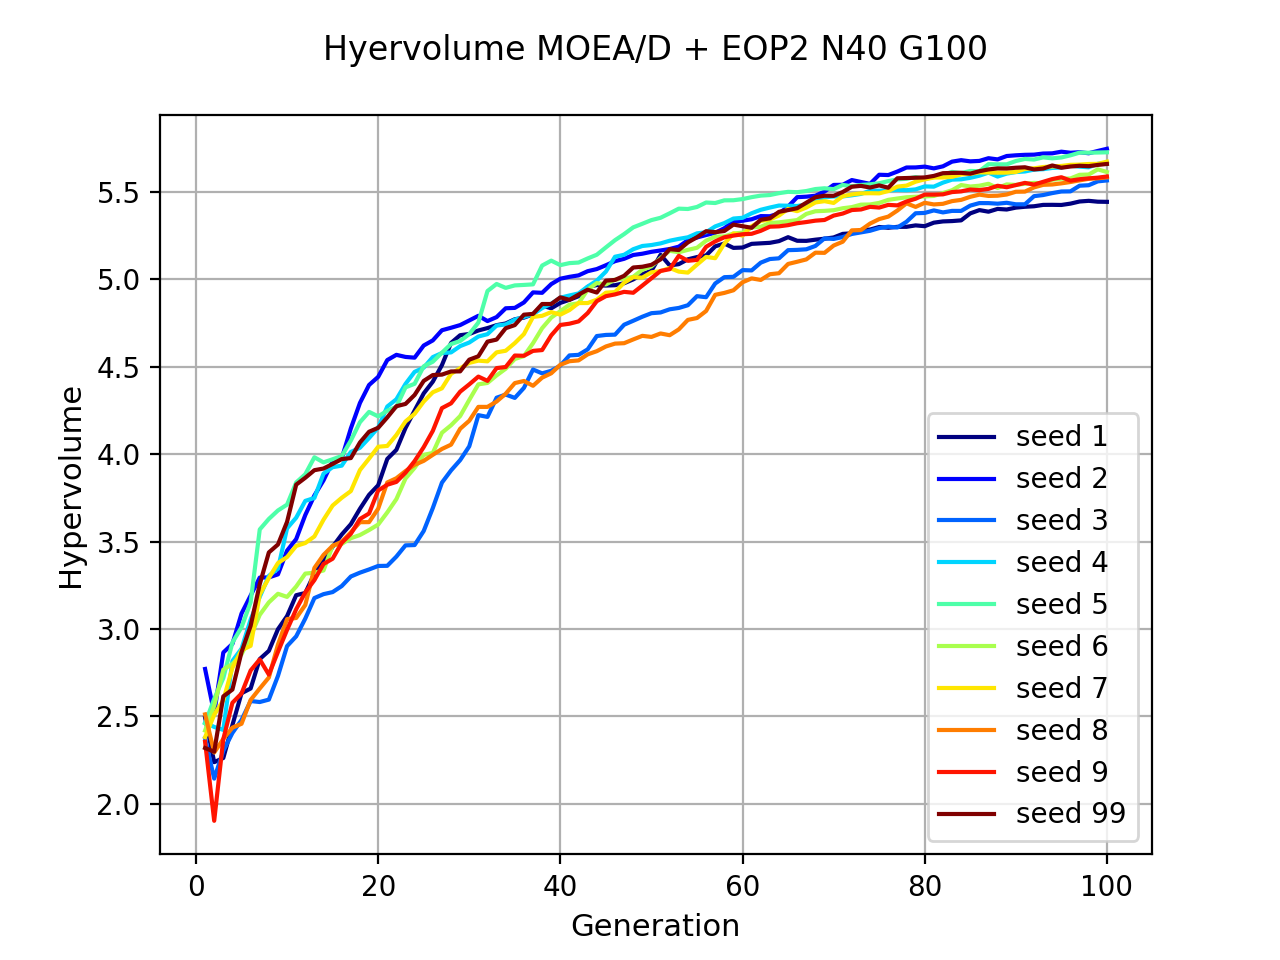
\includegraphics[scale=0.43]{figures/METRICS_EOP2/Hypervol_N40_G100.png} \quad 
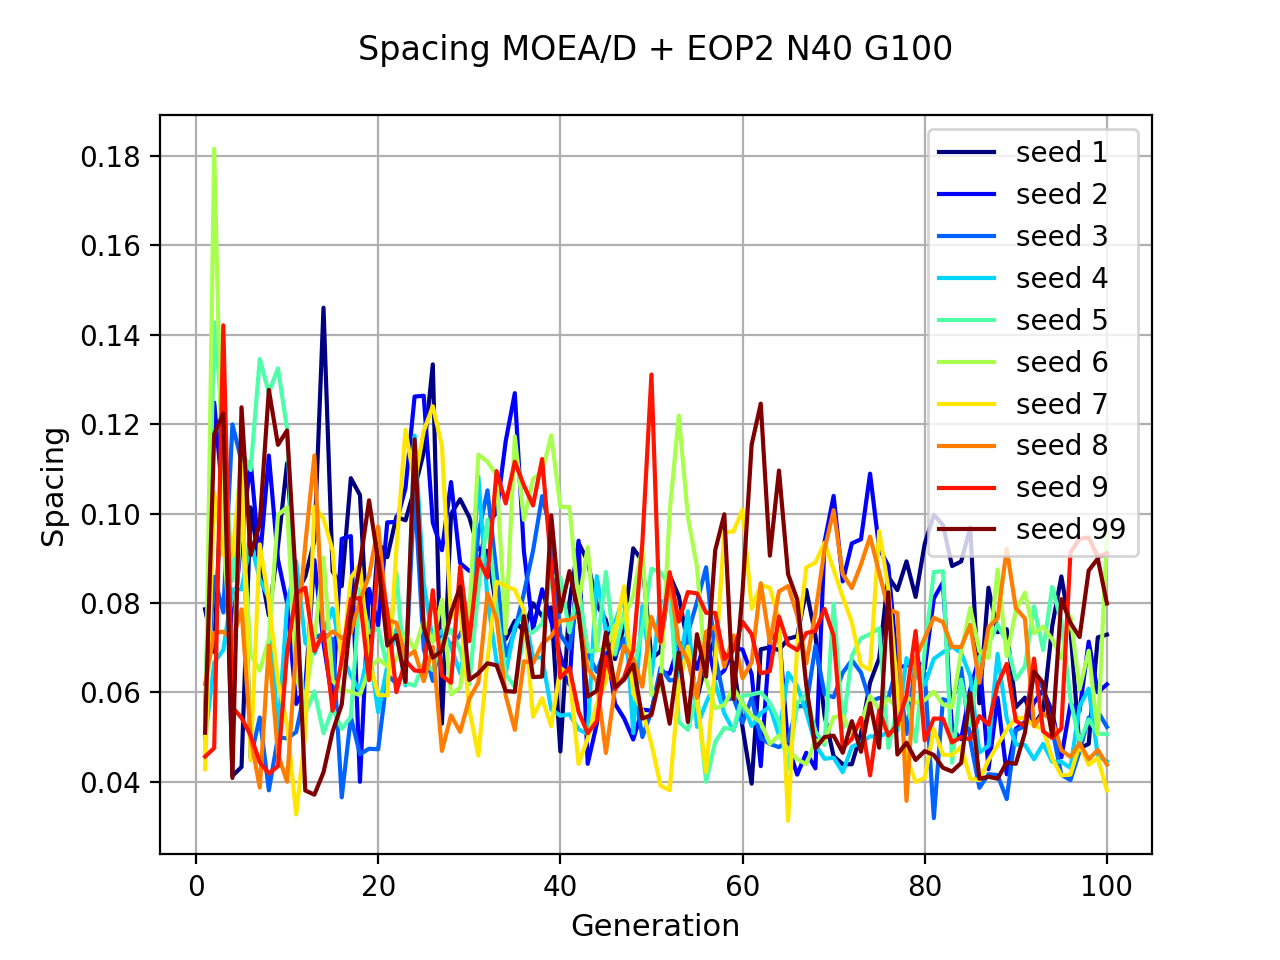
\includegraphics[scale=0.43]{figures/METRICS_EOP2/Spacing_N40_G100.png}\\
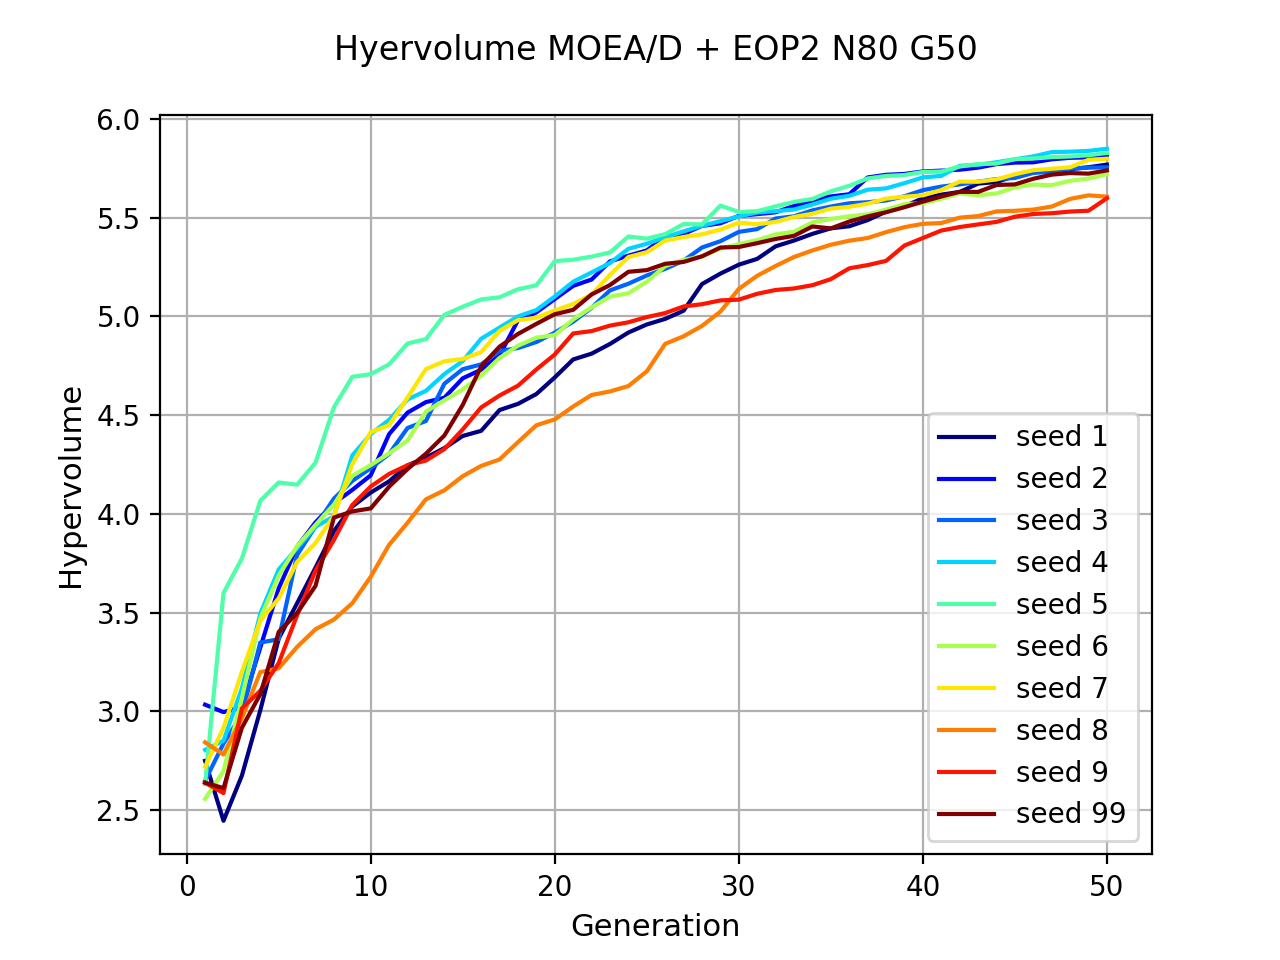
\includegraphics[scale=0.43]{figures/METRICS_EOP2/Hypervol_N80_G50.png}\quad 
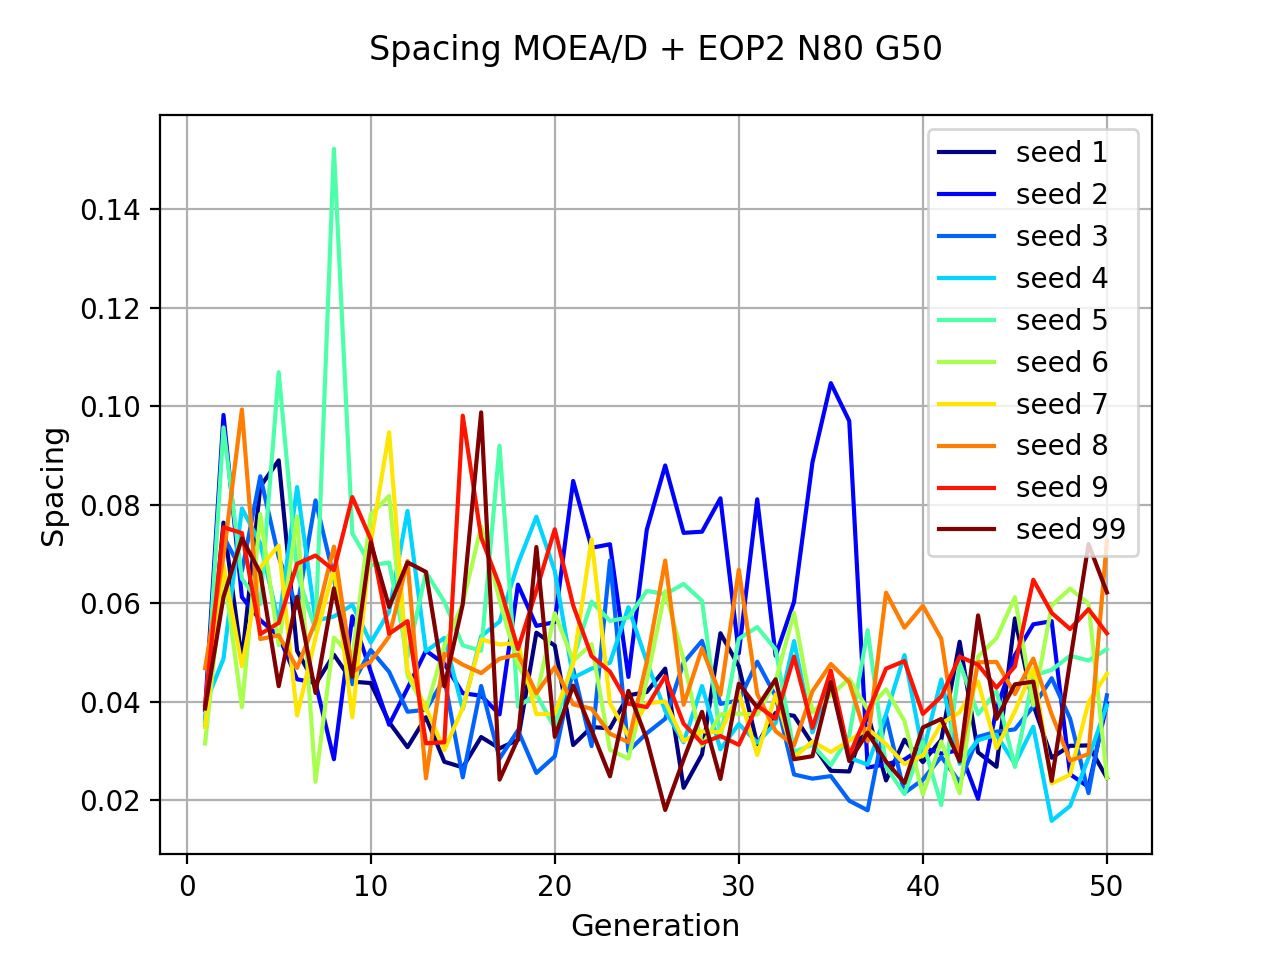
\includegraphics[scale=0.43]{figures/METRICS_EOP2/Spacing_N80_G50.png}\\
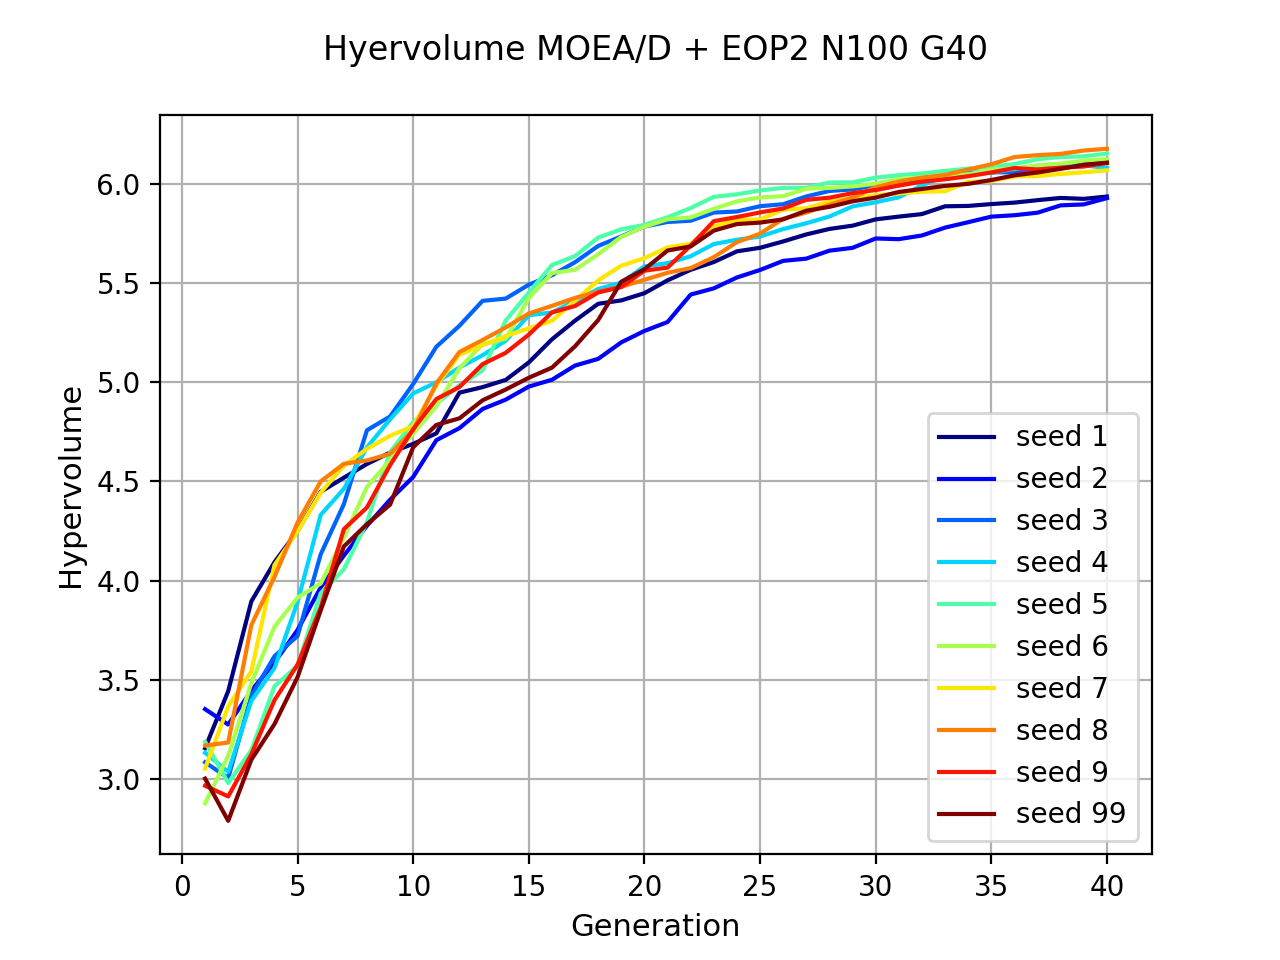
\includegraphics[scale=0.43]{figures/METRICS_EOP2/Hypervol_N100_G40.png}\quad 
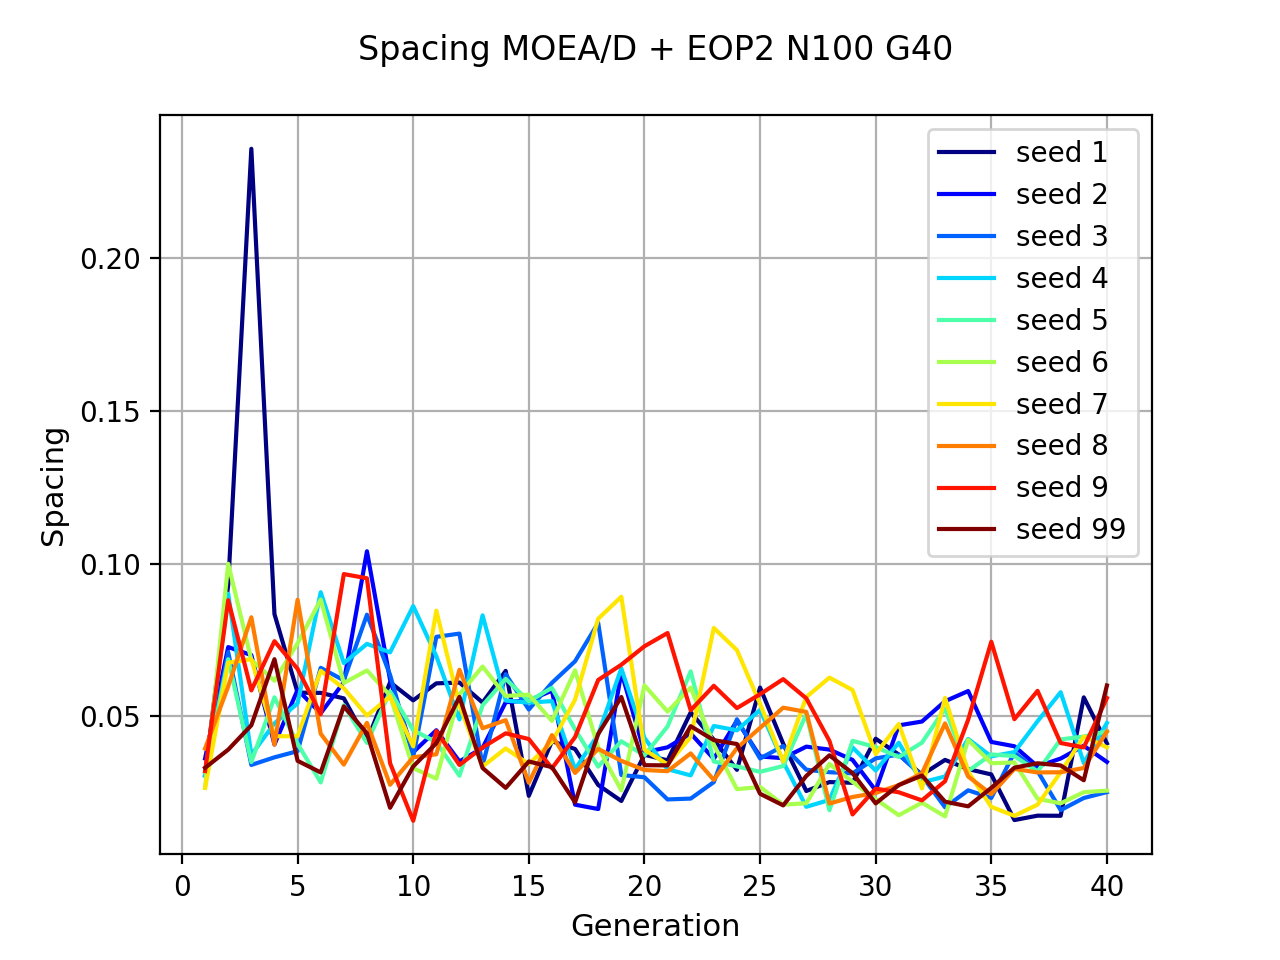
\includegraphics[scale=0.43]{figures/METRICS_EOP2/Spacing_N100_G40.png}\\
\caption{MOEA/D + EOP2. Métricas para 4000EV}
\label{fig:16}
\end{figure}


\begin{figure}[H]
\centering
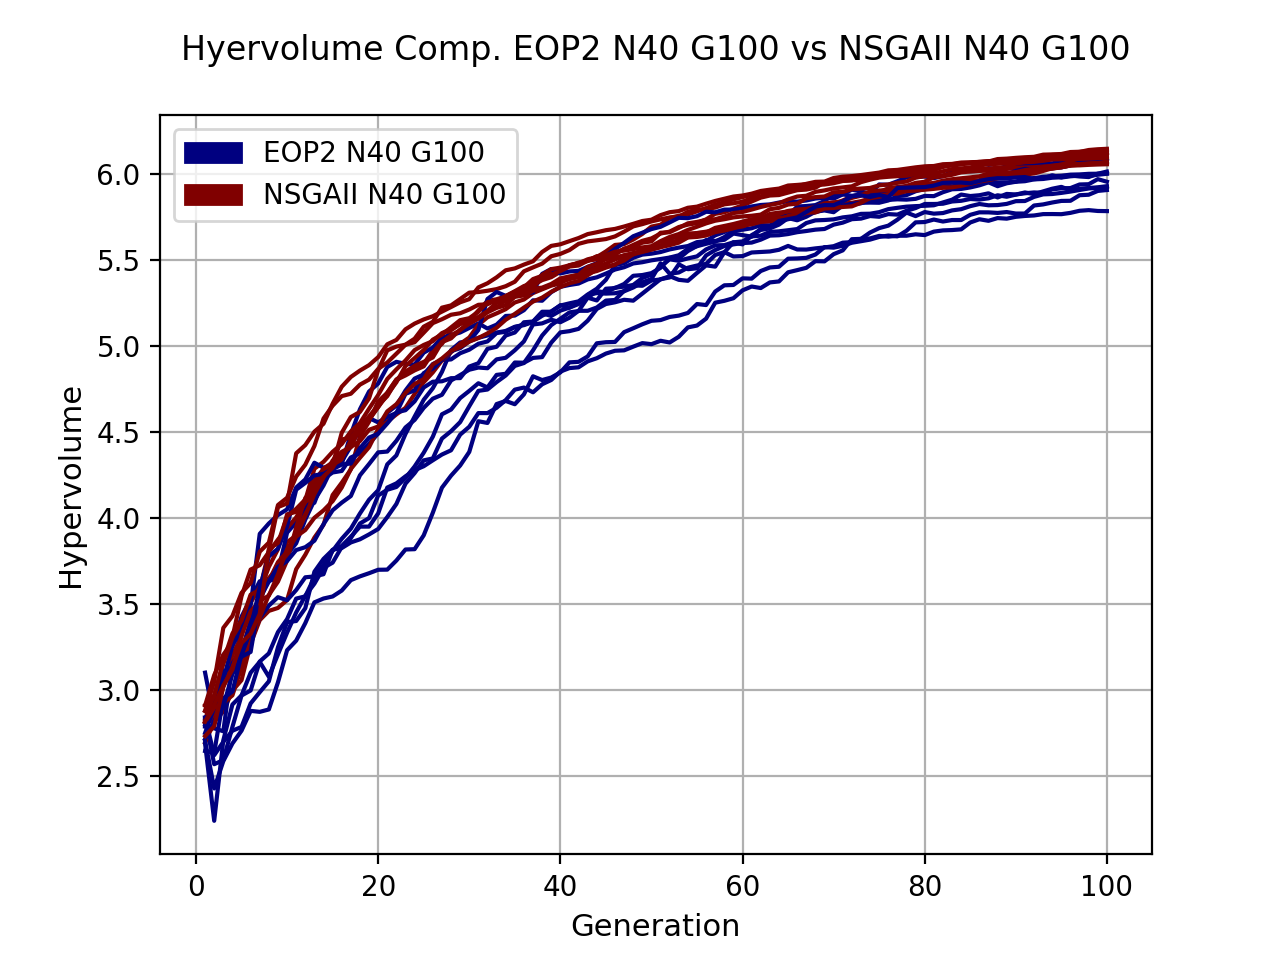
\includegraphics[scale=0.35]{../METRICS_PLOTS/Hypervol_COMP_EOP2N40G100_NSGAIIN40G100.png}
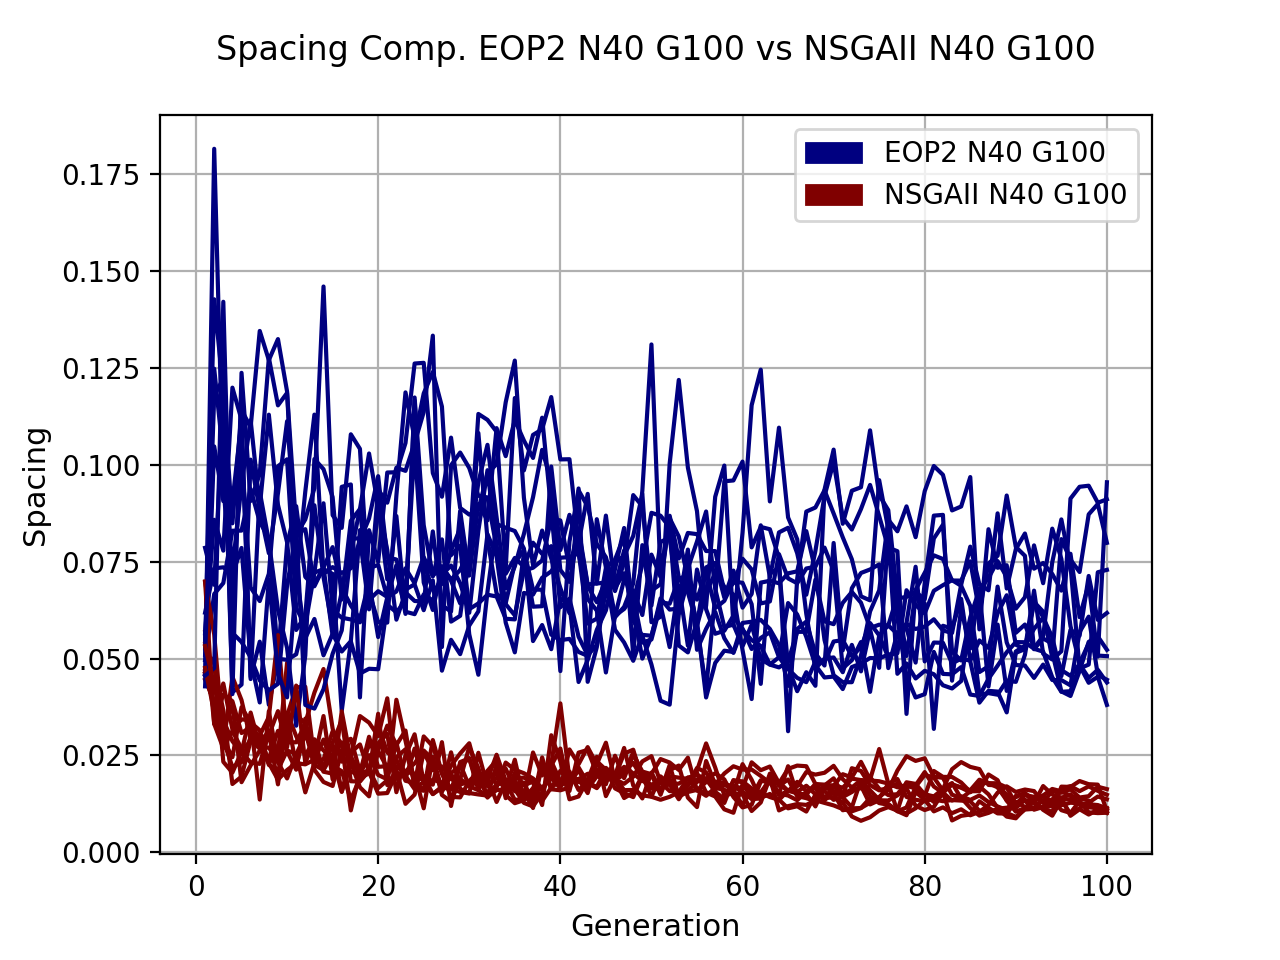
\includegraphics[scale=0.35]{../METRICS_PLOTS/Spacing_COMP_EOP2N40G100_NSGAIIN40G100.png}
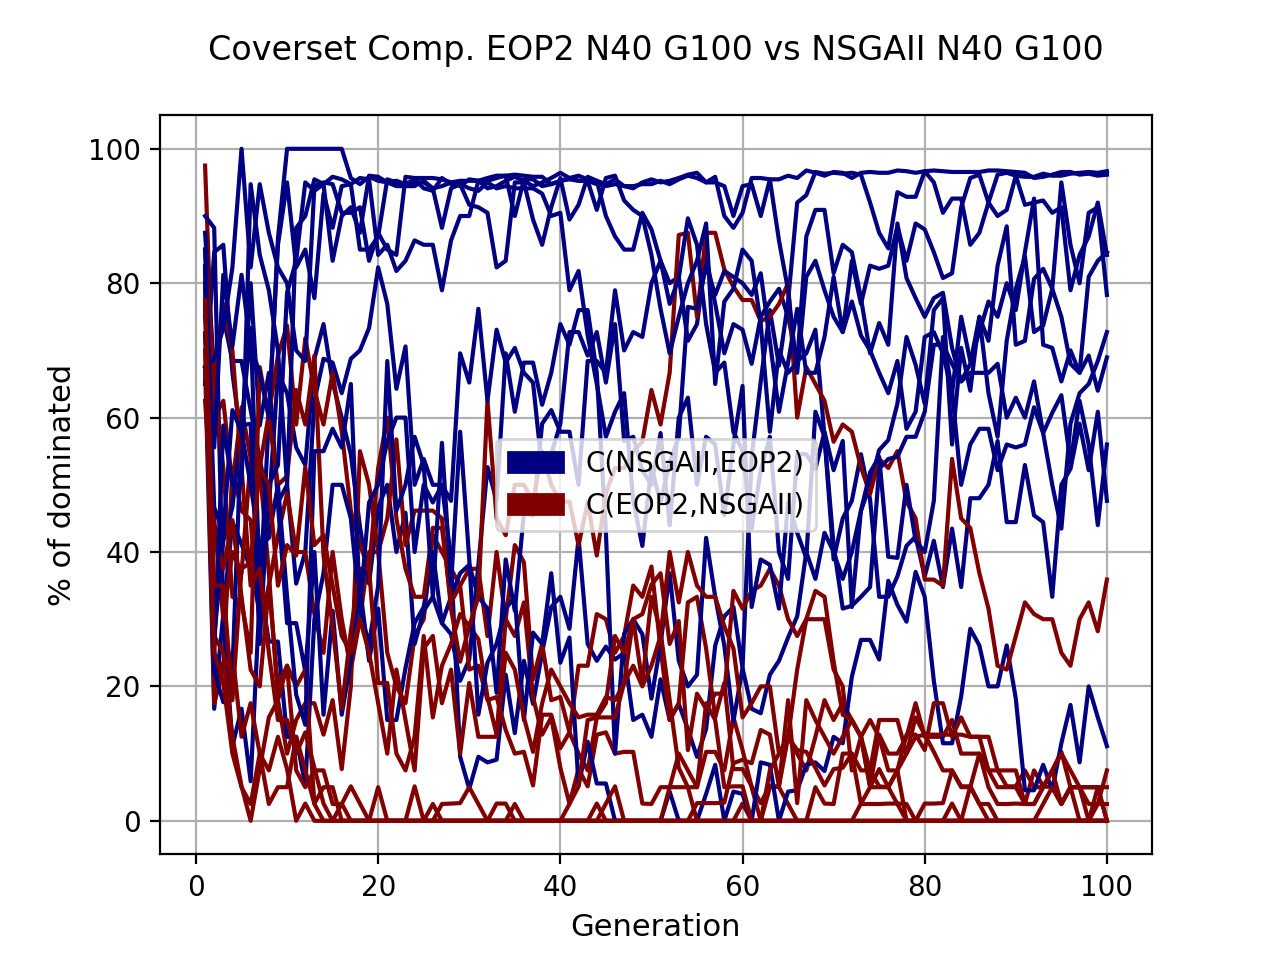
\includegraphics[scale=0.35]{../METRICS_PLOTS/CoverSet_COMP_EOP2N40G100_NSGAIIN40G100.png}\\
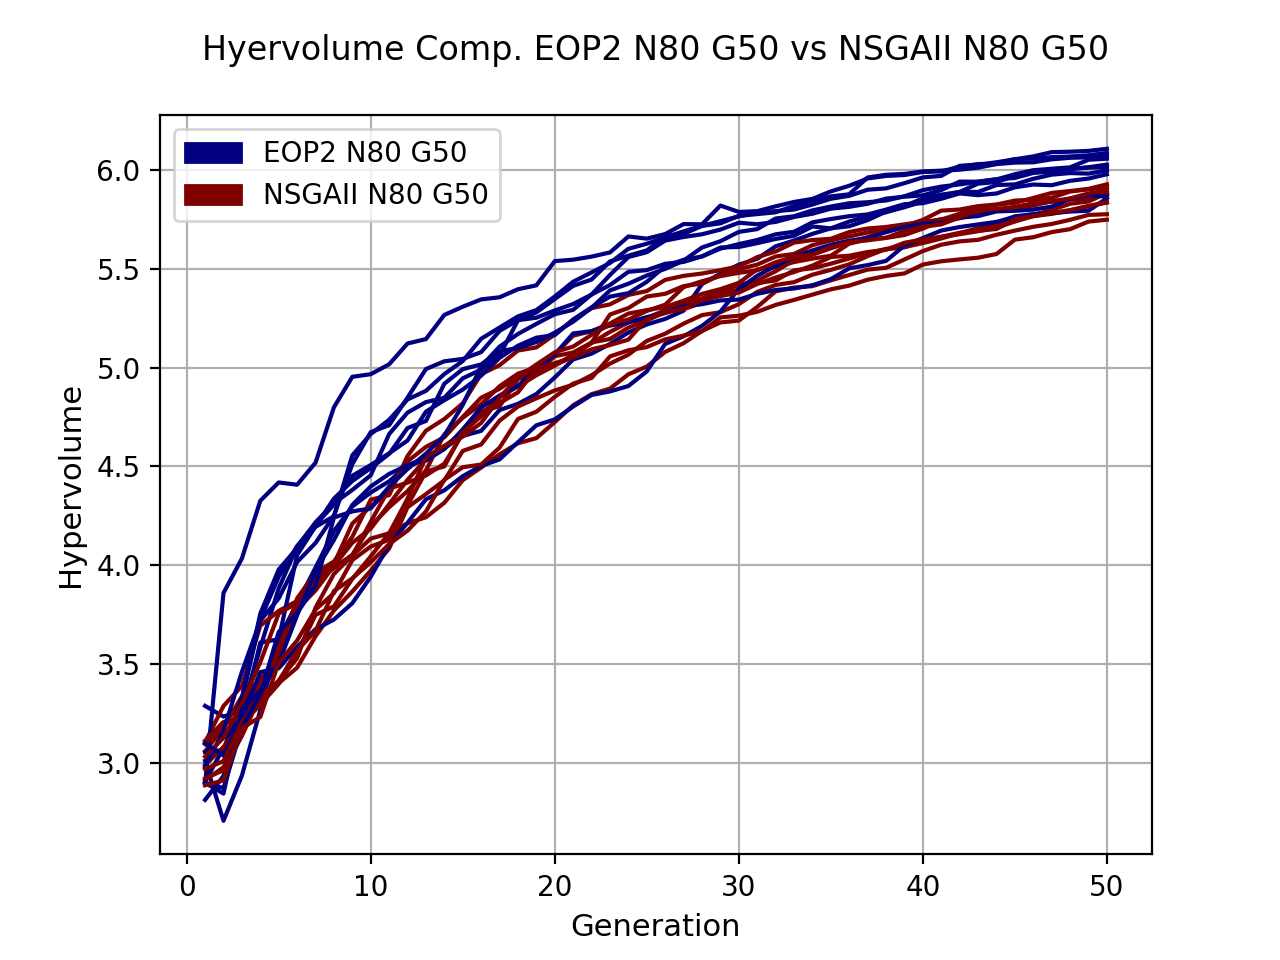
\includegraphics[scale=0.35]{../METRICS_PLOTS/Hypervol_COMP_EOP2N80G50_NSGAIIN80G50.png}
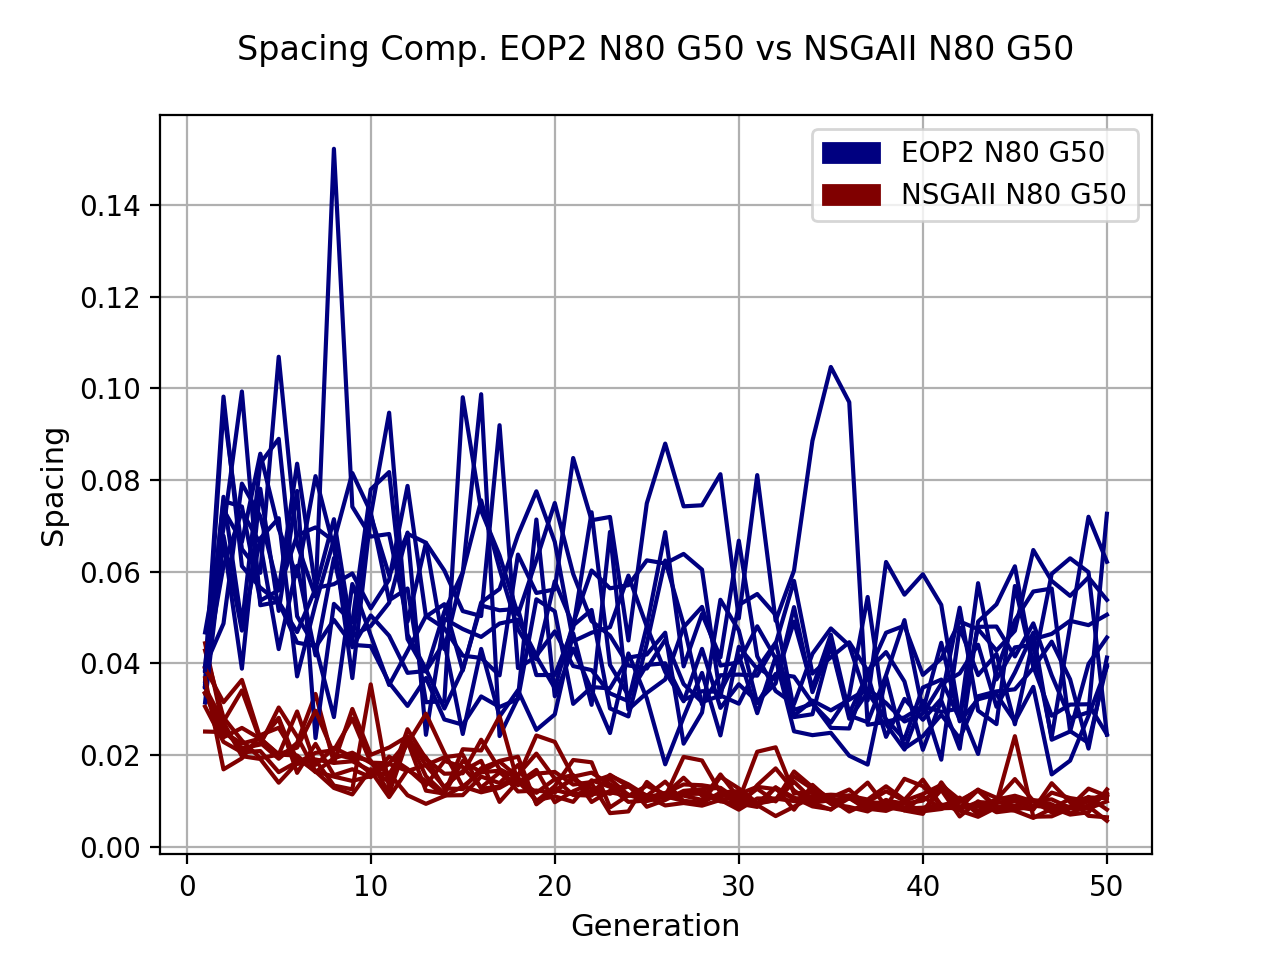
\includegraphics[scale=0.35]{../METRICS_PLOTS/Spacing_COMP_EOP2N80G50_NSGAIIN80G50.png}
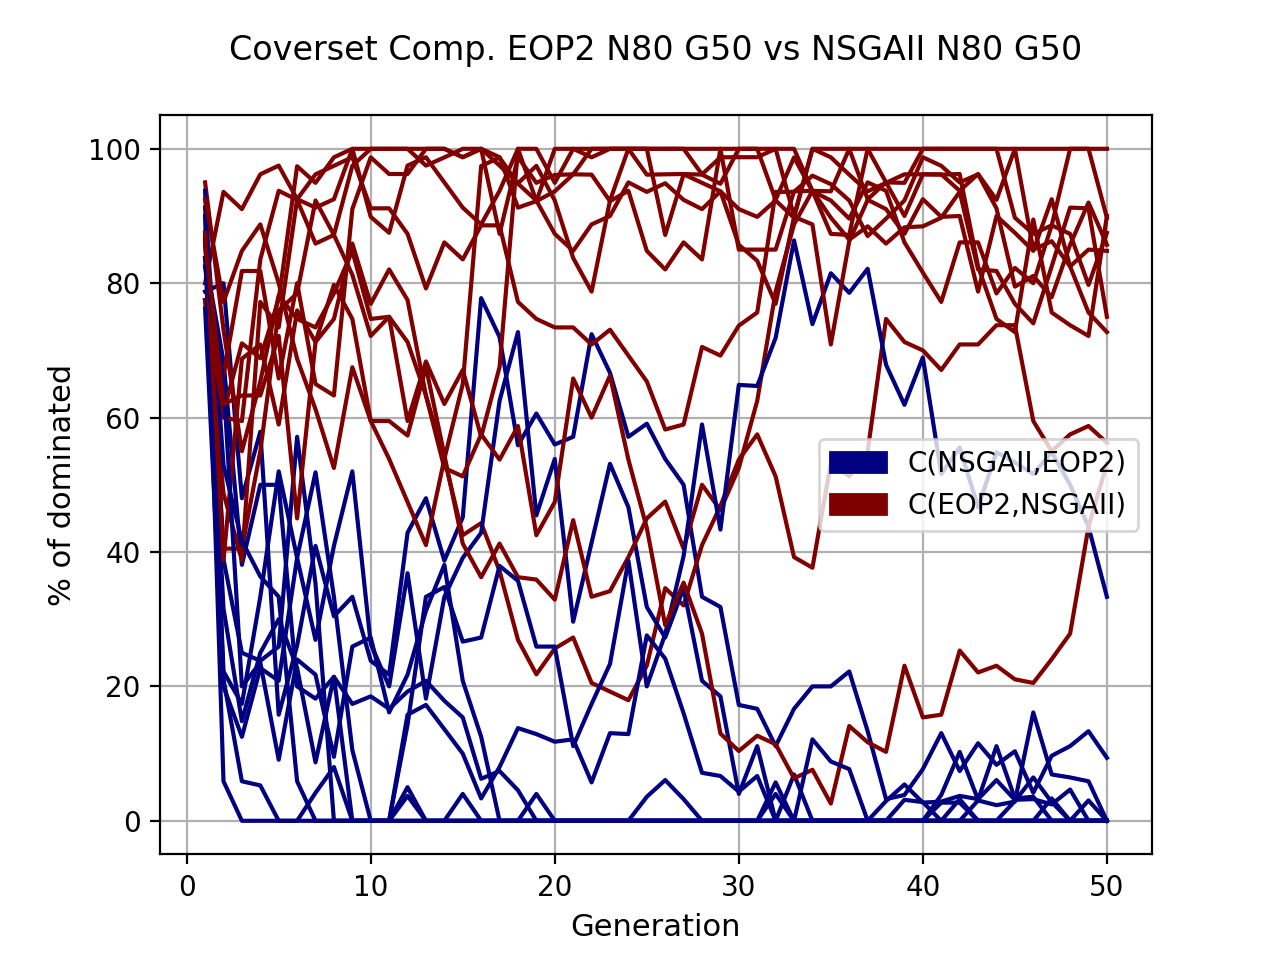
\includegraphics[scale=0.35]{../METRICS_PLOTS/CoverSet_COMP_EOP2N80G50_NSGAIIN80G50.png}\\
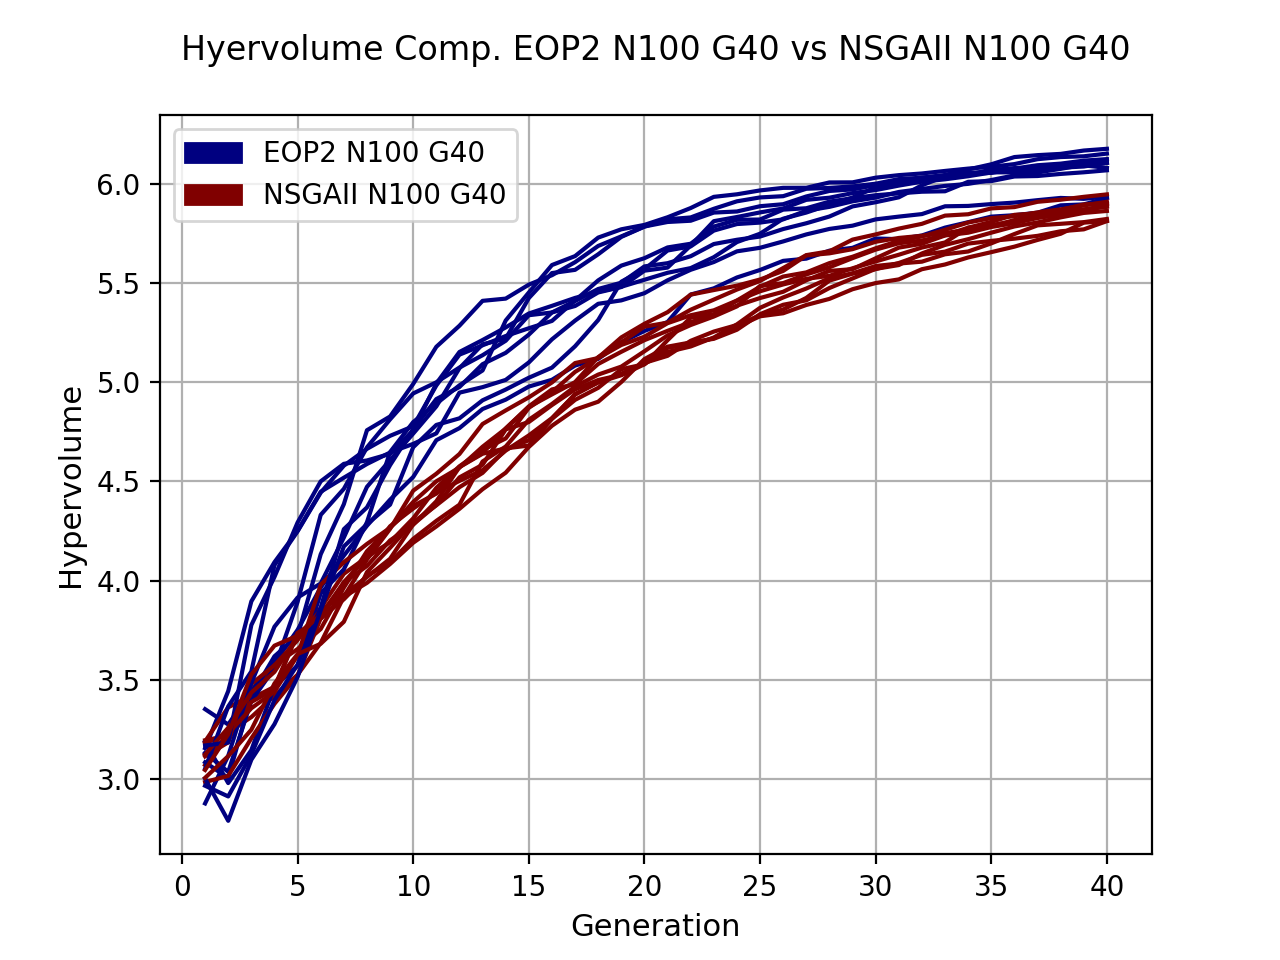
\includegraphics[scale=0.35]{../METRICS_PLOTS/Hypervol_COMP_EOP2N100G40_NSGAIIN100G40.png}
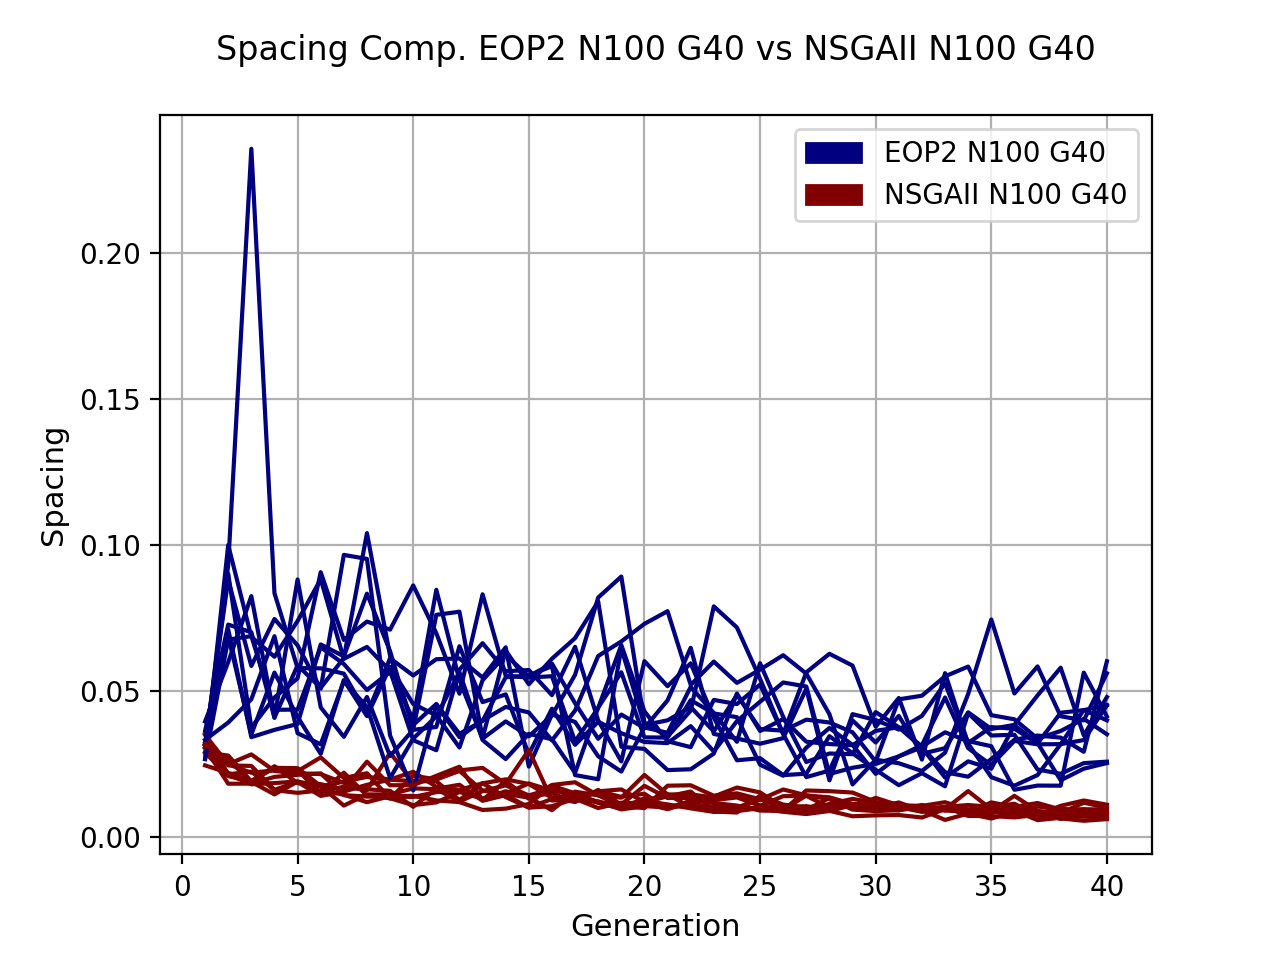
\includegraphics[scale=0.35]{../METRICS_PLOTS/Spacing_COMP_EOP2N100G40_NSGAIIN100G40.png}
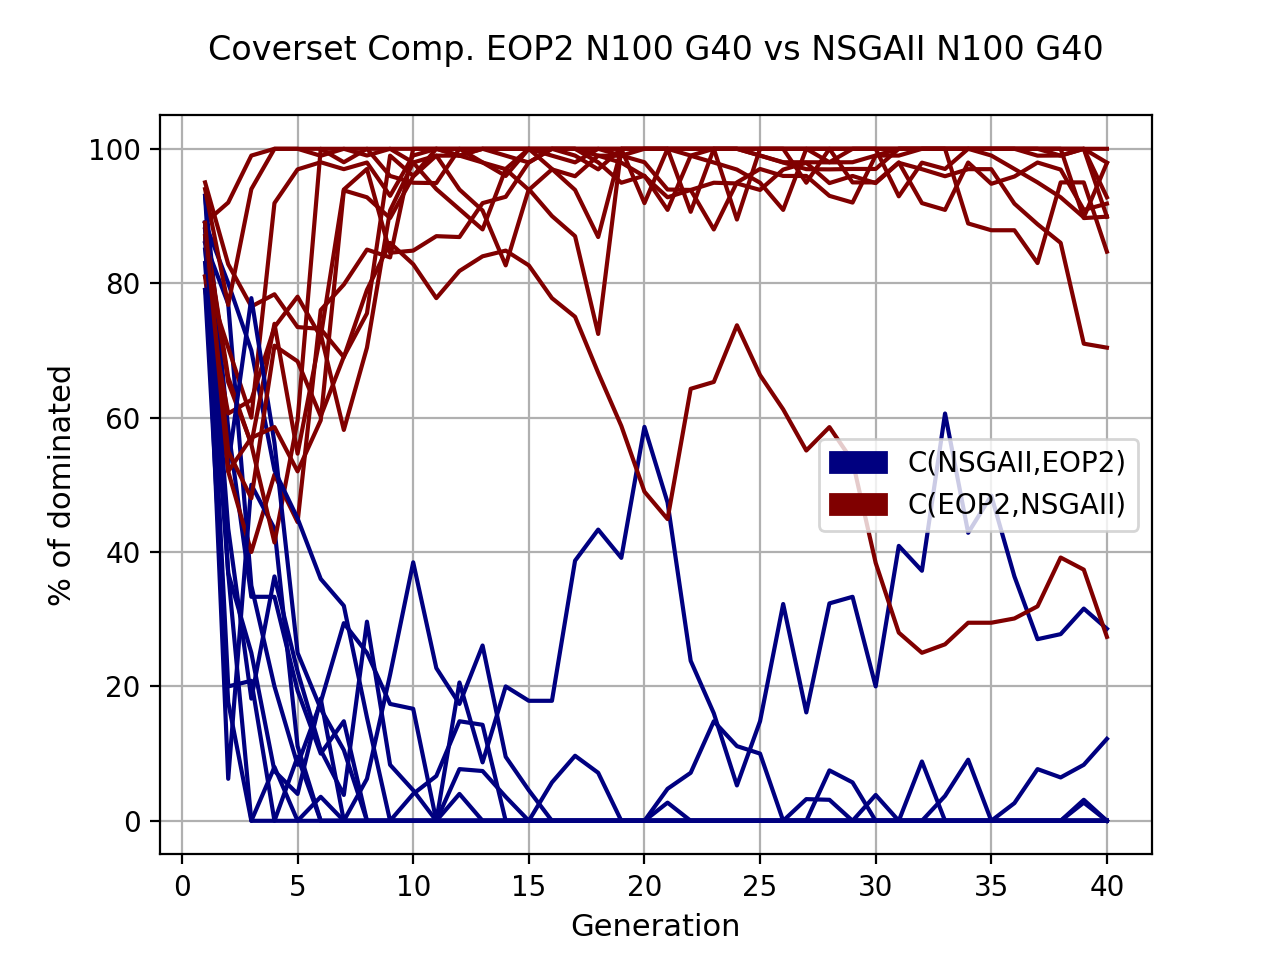
\includegraphics[scale=0.35]{../METRICS_PLOTS/CoverSet_COMP_EOP2N100G40_NSGAIIN100G40.png}\\
\caption{MOEA/D + EOP2. Comparación de métricas con NSGAII para 4000 EV.}
\label{fig:17}
\end{figure}
